\documentclass[12pt,english]{article}
\usepackage[a4paper,left=3cm,right=2cm,top=2.5cm,bottom=2.5cm]{geometry}
\usepackage[utf8]{inputenc}
\usepackage[english]{babel}
\usepackage{graphicx}
\usepackage{pifont}
\usepackage{color}
\usepackage{xcolor}
\usepackage{colortbl}
\usepackage{amsthm,thmtools}
\usepackage{multirow}
\usepackage{pgfgantt}
\usepackage{amsmath}
\usepackage{longtable}
\usepackage{subcaption}
\usepackage{booktabs}
\usepackage{adjustbox}
\usepackage{url}
\usepackage{svg}
\newcommand{\back}[1]{\fontsize{60}{70}\selectfont #1}
\usepackage{multirow}
\usepackage[hidelinks]{hyperref}
\usepackage{caption}
\usepackage[sort&compress, numbers]{natbib}
\definecolor{swotS}{RGB}{226,237,143}
\definecolor{swotW}{RGB}{247,193,139}
\definecolor{swotO}{RGB}{173,208,187}
\definecolor{swotT}{RGB}{192,165,184}
\usepackage{eurosym} % para el euro
\usepackage[raster]{tcolorbox}
\usepackage{amsthm}
\usepackage{multicol}
\usepackage{float}
\usepackage{amsfonts}
\usepackage[usestackEOL]{stackengine}
\usepackage{titling}
\usepackage{soul}
\usepackage{dirtree}
\usepackage{pgfplots}
\usepackage[nottoc]{tocbibind}
\usepackage{listings}
\usepackage{array}
\usepackage[framemethod=tikz]{mdframed}
\usetikzlibrary{matrix, shapes, arrows,calc, positioning, chains, fit, decorations}
\usepackage{footnote}
\newcommand{\dollar}{\mbox{\textdollar}}
\usepackage{lscape}
\usepackage{amsmath}  % for \hookrightarrow
\usepackage{xcolor}   % for \textcolor
\usepackage{incgraph}
\usepackage[toc,page]{appendix}
\makesavenoteenv{tabular}
\makesavenoteenv{table}
\newcommand{\greentick}{\textcolor{green}{\ding{52}}}
\newcommand{\redcross}{\textcolor{red}{\ding{55}}}
\graphicspath{ {./img/}}
\makeatletter
\def\input@path{{input/}}
\makeatother
\selectlanguage{english}
%\usepackage{fancyhdr}
%\pagestyle{fancy}
\usepackage[
    type={CC},
    modifier={by-nc-sa},
    version={4.0},
]{doclicense}
% Default fixed font does not support bold face
\DeclareFixedFont{\ttb}{T1}{txtt}{bx}{n}{10} % for bold
\DeclareFixedFont{\ttm}{T1}{txtt}{m}{n}{10}  % for normal

% Custom colors
\usepackage{color}
\definecolor{deepblue}{rgb}{0,0,0.5}
\definecolor{deepred}{rgb}{0.6,0,0}
\definecolor{deepgreen}{rgb}{0,0.5,0}
% Python style for highlighting
\newcommand\pythonstyle{\lstset{
language=Python,
basicstyle=\ttm,
otherkeywords={self},          % Add keywords here
keywordstyle=\ttb\color{deepblue},
emph={MyClass,__init__},          % Custom highlighting
emphstyle=\ttb\color{deepred},    % Custom highlighting style
stringstyle=\color{deepgreen},
frame=tb,
tabsize=2,
literate={\ \ }{{\ }}1,                        % Any extra options here
showstringspaces=false            %
}}
% Python environment
\lstnewenvironment{python}[1][]
{
\pythonstyle
\lstset{#1}
}
{}

% Python for external files
\newcommand\pythonexternal[2][]{{
\pythonstyle
\lstinputlisting[#1]{#2}}}

% Python for inline
\newcommand\pythoninline[1]{{\pythonstyle\lstinline!#1!}}

\lstdefinelanguage{docker-compose-2}{
  keywords={version, services},
  keywordstyle=[2]\color{blue}\bfseries,
  keywords=[2]{image, environment, ports, container_name, ports, links, build,
  volumes, depends_on, restart},
  keywordstyle=\color{olive}\bfseries,
  identifierstyle=\color{black},
  sensitive=false,
  comment=[l]{\#},
  commentstyle=\color{purple}\ttfamily,
  stringstyle=\color{red}\ttfamily,
  morestring=[b]',
  morestring=[b]"
}

\lstdefinelanguage{docker}{
  keywords={FROM, RUN, COPY, ADD, ENTRYPOINT, CMD,  ENV, ARG, WORKDIR, EXPOSE, LABEL, USER, VOLUME, STOPSIGNAL, ONBUILD, MAINTAINER},
  keywordstyle=\color{blue}\bfseries,
  identifierstyle=\color{black},
  sensitive=false,
  comment=[l]{\#},
  commentstyle=\color{purple}\ttfamily,
  stringstyle=\color{red}\ttfamily,
  morestring=[b]',
  morestring=[b]"
}

\lstdefinelanguage{flutter}{
  keywords={class, extends, final, return, this, async, await, new, final, false, void, true, itemBuilder, onSelected},
  keywordstyle=\color{blue}\bfseries,
  identifierstyle=\color{black},
  sensitive=false,
  comment=[l]{\#},
  commentstyle=\color{purple}\ttfamily,
  stringstyle=\color{red}\ttfamily,
  morestring=[b]',
  morestring=[b]",
  tabsize=2,
  literate={\ \ }{{\ }}1,
}

\colorlet{helpful}{lime!70}
\colorlet{harmful}{red!30}
\colorlet{internal}{yellow!20}
\colorlet{external}{cyan!30}
\colorlet{S}{helpful!50!internal}
\colorlet{W}{harmful!50!internal}
\colorlet{O}{helpful!50!external}
\colorlet{T}{harmful!50!external}

\lstset{
  breaklines=true,
  postbreak=\mbox{\textcolor{red}{$\hookrightarrow$}\space},
  mathescape = true,
  basicstyle=\ttm,
  keywordstyle=\ttb\color{deepblue},
  emph={MyClass,__init__},          % Custom highlighting
  emphstyle=\ttb\color{deepred},    % Custom highlighting style
  stringstyle=\color{deepgreen},
  frame=tb,                         % Any extra options here
  showstringspaces=false,            %
  aboveskip=20pt,
  belowskip=20pt
}

\makeindex

\definecolor{light-gray}{gray}{0.95}
\lstset{columns=fullflexible,basicstyle=\ttfamily}
\newcommand{\texta}{Helpful\\ \tiny (to achieve the objective)\par}
\newcommand{\textb}{Harmful\\ \tiny (to achieve the objective)\par}
\newcommand{\textcn}{Internal origin\\ \tiny (product\slash company attributes)\par}
\newcommand{\textdn}{External origin\\ \tiny (environment\slash market attributes)\par}


\pgfplotsset{width=8cm,compat=1.9, xlabel={Year},
  ylabel={Number of documents}, xtick distance={2},
  ytick distance={2}, ymajorgrids=true,grid style=dashed,
  /pgf/number format/.cd,use comma,1000 sep={}}


\begin{document}

\begin{titlepage}

 \newlength{\centeroffset}
 \setlength{\centeroffset}{-0.5\oddsidemargin}
 \addtolength{\centeroffset}{0.5\evensidemargin}
 \thispagestyle{empty}

 \noindent\hspace*{\centeroffset}
 \begin{minipage}{\textwidth}

  \centering
  
\includegraphics[width=0.9\textwidth]{logo_ugr.jpg}\\[1.4cm]

  \textsc{ \Large Bachelor Thesis\\[0.2cm]}
  \textsc{Computer Engineering}\\[1cm]

  {\Huge\bfseries Are-U-Drunk?\\}
  \noindent\rule[-1ex]{\textwidth}{3pt}\\[3.5ex]
  {\large\bfseries Measuring alcohol intoxication via smart mobile sensing}
 \end{minipage}

 \vspace{1cm}
 \noindent\hspace*{\centeroffset}
 \begin{minipage}{\textwidth}
  \centering

  \textbf{Author}\\ {Cristina Díaz García}\\[2.5ex]
  \textbf{Supervisors}\\
  {Oresti Baños Legrán}\\
  {Claudia Villalonga Palliser}\\[3ex]
  
\includegraphics[width=0.4\textwidth]{etsiit_logo.png}\\[0.1cm]
  \vspace{1cm}
  \textsc{Escuela Técnica Superior de Ingenierías Informática y de Telecomunicación}\\
  \vspace{1cm}
  \textsc{Granada, academic year 2020-2021}
 \end{minipage}
\end{titlepage}


\cleardoublepage
\thispagestyle{empty}

\begin{center}
{\large\bfseries Are-U-Drunk? Measuring alcohol intoxication via smart mobile sensing}\\
\end{center}
\begin{center}
Cristina Díaz García\\
\end{center}

%\vspace{0.7cm}
\noindent{\textbf{Palabras clave}: alcohol, desarrollo móvil, procesamiento de video}\\

\vspace{0.7cm}
\noindent{\textbf{Resumen}}\\

El alcohol es una droga legal de la que a veces se hace un uso excesivo y/o inadecuado. Esto no solo puede afectar a quien la usa, sino a quien le rodea, ya que el comportamiendo del sujeto puede llevar a situaciones como una pelea o un accidente de tráfico. El objetivo de este proyecto es la detección de un posible abuso del alcohol para así poder informar al usuario y facilitar una toma de mejores decisiones. Es por ello que se ha diseñado un sistema digital de detección de movimiento ocular con el que detectar movimientos involuntarios provocados por el efecto del alcohol en el sistema nervioso. La usabilidad y el rendimiento de la aplicación desarrollada han sido evaluados mediante una escala de usabilidad de sistemas, System Usability Scale en inglés, en la que se puntúan diferentes aspectos del sistema. Tras esta evaluación, la aplicación ha demostrado ser útil, usable y práctica.

\cleardoublepage


\thispagestyle{empty}


\begin{center}
{\large\bfseries Are-U-Drunk? Measuring alcohol intoxication via smart mobile sensing}\\
\end{center}
\begin{center}
Cristina Díaz García \\
\end{center}

%\vspace{0.7cm}
\noindent{\textbf{Keywords}: alcohol, mobile, video processing}\\

\vspace{0.7cm}
\noindent{\textbf{Abstract}}\\

Alcohol is a legal drug that is sometimes overused and/or misused. This can affect not only who uses it, but who surrounds them, since the behavior of the subject can lead to situations such as a fight or a traffic accident. The objective of this project is the detection of possible alcohol abuse in order to inform the user and facilitate better decision-making. For this purpose a digital eye movement detection system has been designed with which to detect involuntary movements caused by the effect of alcohol on the nervous system. The usability and performance of the developed application have been evaluated using a System Usability Scale, in which different aspects of the system are scored. After this evaluation, the application has proven to be useful, usable and practical.

\newpage

\section*{}
\thispagestyle{empty}

\noindent\rule[-1ex]{\textwidth}{2pt}\\[4.5ex]

Yo, \textbf{Cristina Díaz García}, estudiante de la titulación Graduado en Ingeniería Informática de la \textbf{Escuela Técnica Superior
de Ingenierías Informática y de Telecomunicación de la Universidad de Granada}, con DNI 53742687J, autorizo la
ubicación de la siguiente copia de mi Trabajo Fin de Grado en la biblioteca del centro para que pueda ser
consultada por las personas que lo deseen.

\vspace{6cm}

\begin{center}
  Fdo: Cristina Díaz García

\end{center}

\vspace{2cm}

\begin{flushright}
Granada a 06 de septiembre de 2021
\end{flushright}

\newpage

\section*{}
\thispagestyle{empty}

\noindent\rule[-1ex]{\textwidth}{2pt}\\[4.5ex]

D. \textbf{Oresti Baños Legrán} y Dª. \textbf{Claudia Villalonga Palliser}, ambos profesores del Departamento Arquitectura de Computadores de la Universidad de Granada.



\vspace{0.5cm}

\textbf{Informa:}

\vspace{0.5cm}

Que el presente trabajo, titulado \textit{\textbf{Are-U-Drunk? Measuring alcohol intoxication via smart mobile sensing}},
ha sido realizado bajo su supervisión por \textbf{Cristina Díaz García}, y autorizo la defensa de dicho trabajo ante el tribunal
que corresponda.

\vspace{0.5cm}

Y para que conste, expide y firma el presente informe en Granada a 06 de septiembre de 2021

\vspace{1cm}

\textbf{El supervisor:}

\vspace{5cm}
\begin{center}
\textbf{Oresti Baños Legrán}

\end{center}

\textbf{La supervisora:}

\vspace{5cm}
\begin{center}
\textbf{Claudia Villalonga Palliser}

\end{center}


\newpage

\section*{Agradecimientos}
\thispagestyle{empty}

\vspace{1cm}
\begin{flushleft}
A mi padre, mi madre y mi hermano, que me han inculcado los valores que tengo y me han hecho llegar hasta donde estoy.\\

A Carlos, por estar siempre ahí.\\

A mis amigos y amigas, especialmente Casandra y Francisco, por ser puntos de apoyo incondicionales cuando más falta hace.
\end{flushleft}

\thispagestyle{empty}
\newpage
\tableofcontents{}
\newpage
\listoffigures
\newpage
\listoftables
\newpage
\lstlistoflistings
\newpage
%\thispagestyle{empty}
%\newpage
%\rhead{}
%\lhead{}
%\renewcommand{\headrulewidth}{0pt}
%\renewcommand{\footrulewidth}{0pt}

\section{Introduction}

\subsection{Context}

Alcohol is a legal drug in most countries worldwide, which makes it very easy to access for anyone who is over the legal age to buy it in their country.

According to organizations like the World Health Organization \cite{who}, the harmful use of alcohol is a causal factor in more than 200 disease and injury conditions and in the age group 20–39 years approximately 13.5\% of the total deaths are alcohol-attributable. Worldwide, 3 million deaths every year result from the harmful use of alcohol, a 5.3\% of all deaths \cite{whoalcohol}.

As it is shown in Figure \ref{vulnerabilities}, there are individual and societal vulnerability factors \cite{whoalcohol} that affect alcohol consumption and alcohol-related harm. In the context of the occidental world, alcohol consumption is totally accepted and most of the socialization among individuals is made by eating and drinking, being most of the beverages alcoholic ones. This could lead sometimes to a misuse and abuse of alcoholic beverages, taking bad decisions, some more naive like texting an ex-partner, some more hazardous like driving.

\begin{figure}[H]
    \centering
    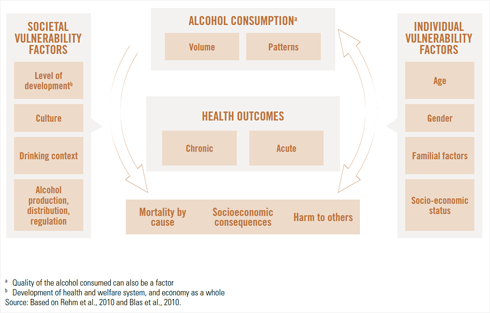
\includegraphics[width=0.9\textwidth]{./img/vulnerabilities.png}
    \caption{Vulnerabilities declared by the WHO. Reprinted from \cite{who}.}
    \label{vulnerabilities}
\end{figure}

  \subsection{Motivation}

  Nowadays, most people, at least in the developed countries, own one or more smartphones. This makes the monitoring of people easier than ever. Adding to this fact how science has advanced, it makes up one of the best possible scenarios for studying the interaction between society and alcohol intake, both amount of alcohol consumed and behavior changes.

  Having in mind what has been previously mentioned and with the exhaustive use of smartphones that is being done, the sensing of people's behaviors has been made easier, and as an example, we could use the keyboard to check whether the writing gets worse or the predictive words are used more frequently after consuming alcohol or taking a selfie to estimate the blood alcohol concentration.

  According to Medical News Today \cite{mnt} and Healthline \cite{healthline}, amoung the numerous effects on the consumer's body and behaviour, the consumption of alcohol may lead to reduced reaction and movement. This will be key aspect to be considered for the system we want to develop. As a consequence of the alcohol intoxication, an abnormal movement is shown by the eyes, known as Nystagmus.

  Nystagmus is, according to MedlinePlus \cite{Nystagmus}, 'a term to describe fast, uncontrollable movements of the eyes that may be side to side (horizontal nystagmus), up and down (vertical nystagmus) and rotary (rotary or torsional nystagmus)'. This effect is the one described in Figure \ref{nystagmuses}. Nystagmus can affect vision, balance, and coordination.

  \begin{figure}[H]
      \centering
      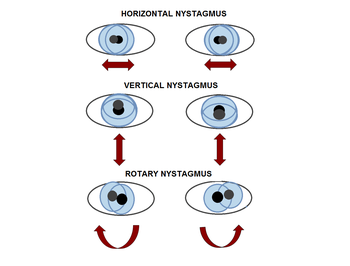
\includegraphics[width=0.45\textwidth]{./img/nystagmuses.png}
      \caption{Horizontal, vertical and rotary Nystagmus}
      \label{nystagmuses}
  \end{figure}

  \subsection{Approach and planning}


  \subsection{Objectives}
  \begin{itemize}
    \item \textbf{Main goal}: to develop a system to automatically assess a person's drunkness based on the analysis of their eye(s) movement.
    \item \textbf{Secondary goals}:
      \begin{itemize}
        \item To design a system that detects and tracks the user's eyes and analyzes them in search of horizontal nystagmus movements.
        \item To develop a system that detects and tracks the user's eyes and analyzes them in search of horizontal nystagmus movements.
        \item To evaluate and test the previously mentioned system.
      \end{itemize}
  \end{itemize}

  \subsection{Structure}

The first chapter of the project, \textit{\nameref{state}}, contains a wider perspective of the current state of tools to detect and monitorize alcohol consumption through a research about wearables, applications and scientific articles. The second chapter, \textit{\nameref{design}}, shows a more exhaustive list of the requisites of the system and the design followed: architecture, programming languages and frameworks used. The third chapter, \textit{\nameref{implementation}}, offers a detailed explanation of the development and deployment of the system. The fourth chapter, \textit{\nameref{discussion}}, analyses the system by means of System Usability Scale tests \cite{sus} and analysis of the data obtained from the use of the application. The fifth and last chapter, \textit{\nameref{conclusions}}, analyses the initial objectives of the project and whether they were achieved or not, as well as possible future work.

\newpage
\section{State of the art}
\label{state}

To get some perspective of the current state of the art with respect to applications related to alcohol intake, three different approaches were taken.

\subsection{Search methods}

\subsubsection{Handsearch}

Some exploration on Google has been done on the field of wearables, such as BACtrack Skyn \cite{bactrackskyn} and Copilot \cite{copiloto}. A later section will deepen on these two wearables.

\subsubsection{Commercial applications}

Firstly, a search through the Apple Store \cite{applestore} was done with three different queries: alcohol, driving, and intake. No applications related to alcohol consumption were found with any of the queries, only driving games and applications to consume more water or measure the intake of calories.
Secondly, a search through the Google Play Store \cite{googleplay} was done with the query alcohol, which threw very interesting results. These results will be reviewed deeper in a later section.

\subsubsection{Scientific publications}

When searching, the terms taken into account were smartphone or similar devices, alcohol or drunkenness and monitor/monitoring and similar. The fields of research were medicine, engineering, psychology and computation. The query used is the one Figure \ref{scopusquery} shows, which threw 231 results on 8th March 2021.

\begin{figure}[h!]
  TITLE-ABS-KEY ( ( smartphone  OR  wearable  OR  smartwatch )  AND  ( alcohol  OR  drunkenness )  AND  ( monitor*  OR  sens*  OR  detect* ) )  AND  ( LIMIT-TO ( PUBYEAR ,  2021 )  OR  LIMIT-TO ( PUBYEAR ,  2020 )  OR  LIMIT-TO ( PUBYEAR ,  2019 )  OR  LIMIT-TO ( PUBYEAR ,  2018 )  OR  LIMIT-TO ( PUBYEAR ,  2017 ) )  AND  ( LIMIT-TO ( SUBJAREA ,  "MEDI" )  OR  LIMIT-TO ( SUBJAREA ,  "ENGI" )  OR  LIMIT-TO ( SUBJAREA ,  "COMP" )  OR  LIMIT-TO ( SUBJAREA ,  "PSYC" ) )
  \caption{Query used in the search through Scopus \cite{scopus}}
  \label{scopusquery}
\end{figure}

Those 231 results were filtered, firstly by the abstract, depending on how interesting the abstract was. This resulted in 63 results after the first filter. These 63 results were once again filtered depending on the accuracy of the abstract according to the subject of our work. Finally,  22 final results were obtained, which were read and a ‘State of Art Matrix’ was built. This matrix can be found in Appendix \ref{appendix:matrix}. After reading the 22 papers, as of 8th March 2021, some very interesting approaches can be analyzed. This proccess is what Figure \ref{proccess} shows.

\begin{figure}[H]
  \centering
  \begin{tikzpicture}
  % NODES
  \tikzset{set/.style={draw,rectangle,inner sep=0pt,align=center}, node distance=1.5cm, minimum height=1cm,minimum width=10cm}
  \node [text centered, rectangle, fill=red!12, draw, rounded corners] (n1) { \textbf{231} unfiltered results (8th March 2021) };
  \node [text centered, rectangle, draw, fill=yellow!20, rounded corners] (n2) [below= of n1]{ \textbf{63} filtered results by interest of abstract };
  \node [text centered, rectangle, draw, fill=green!20, rounded corners] (n3) [below= of n2] { \textbf{22} final results filtered by accuracy of abstract };

  % ARROWS
  \draw [thick,-stealth] (n1) -- node [right,minimum width=1cm] {Filter by abstract} (n2);
  \draw [thick,-stealth] (n2) -- node [right,minimum width=1cm] {Filter by content} (n3);

  \end{tikzpicture}
  \caption{State of the art filtering steps}
  \label{proccess}
\end{figure}

\subsection{Wearables}

BACtrack Skyn \cite{bactrackskyn} is a wearable, a smart bracelet, only available for research, that tracks Transdermal Alcohol Content (TAC) in real time. It can be used on its own or integrated with Apple Watch \cite{applewatch}. It has a cloud-based web portal used to manage, view and export the data obtained with the device. More information can be requested to the BACtrack team on their webpage.

Copilot \cite{copiloto} is a watch and application tandem that allows the user to monitor and learn their driving patterns so it can detect when the pattern changes because of alcohol intake thanks to the watch’s gyroscope, accelerometer and heartbeat monitor.


\subsection{Applications}

As previously mentioned, none of the results when searching through the Google Play \cite{googleplay} were interesting. On the other hand, it is interesting to deepen on the results of the search through the Google Play \cite{googleplay}. The next paragraphs deepen on these results.

\begin{figure}[H]
  \centering
  \begin{subfigure}{0.3\textwidth}
      \centering
      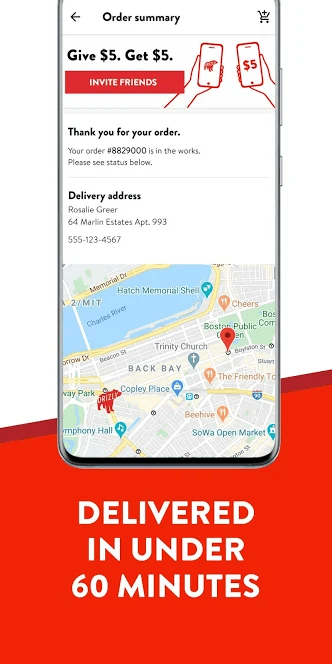
\includegraphics[width=0.8\textwidth]{./img/Drizly.png}
      \caption{Drizly \cite{Drizly} application}
      \label{Drizly}
  \end{subfigure}\hfill
  \begin{subfigure}{0.38\textwidth}
      \centering
      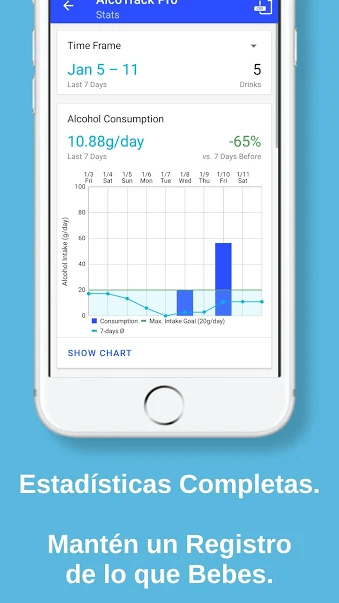
\includegraphics[width=0.8\textwidth]{./img/Alcotrack.png}
      \caption{Alcotrack \cite{alcotrack} application}
      \label{Alcotrack}
  \end{subfigure}
  \begin{subfigure}{0.3\textwidth}
      \centering
      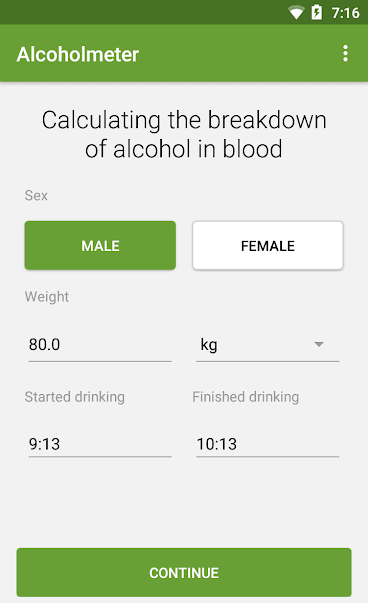
\includegraphics[width=0.8\textwidth]{./img/Alcoholcheck.png}
      \caption{Alcoholcheck \cite{alcoholcheck} application}
      \label{Alcoholcheck}
  \end{subfigure}

%//

  \begin{subfigure}{0.3\textwidth}
      \centering
      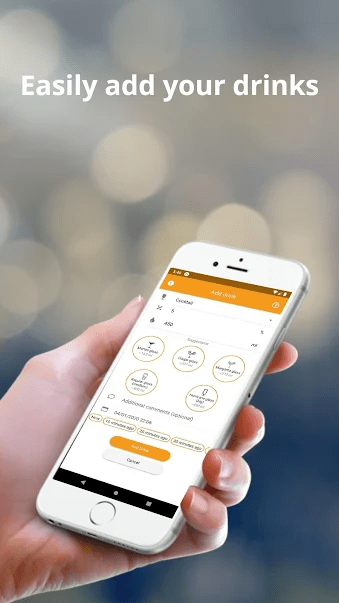
\includegraphics[width=0.65\textwidth]{./img/alcofy.png}
      \caption{Alcofy \cite{Alcofy} application}
      \label{Alcofy}
  \end{subfigure}\hfill
  \begin{subfigure}{0.38\textwidth}
      \centering
      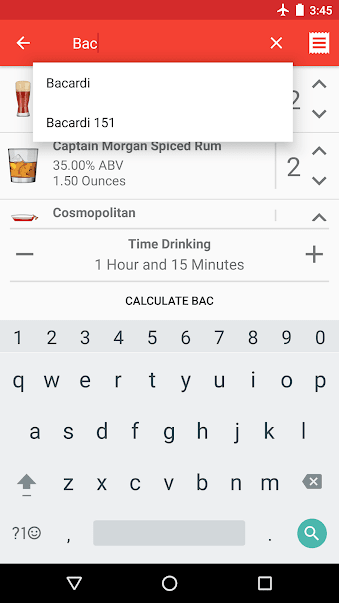
\includegraphics[width=0.5\textwidth]{./img/alcoholcalculator.png}
      \caption{Blood Alcohol Calculator \cite{alcoholcalculator} application}
      \label{alcoholcalculator}
  \end{subfigure}
  \begin{subfigure}{0.3\textwidth}
      \centering
      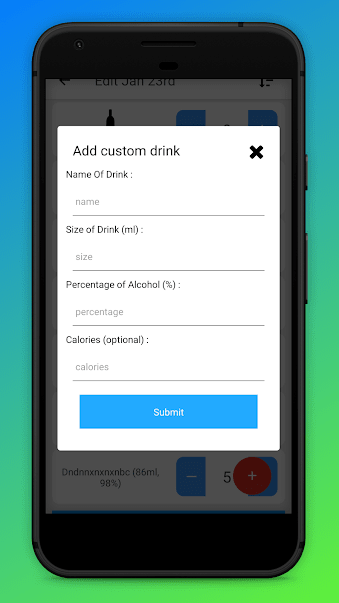
\includegraphics[width=0.65\textwidth]{./img/saut.png}
      \caption{Simple Alcohol Unit Tracker \cite{saut} application}
      \label{saut}
  \end{subfigure}

%//

  \begin{subfigure}{0.3\textwidth}
      \centering
      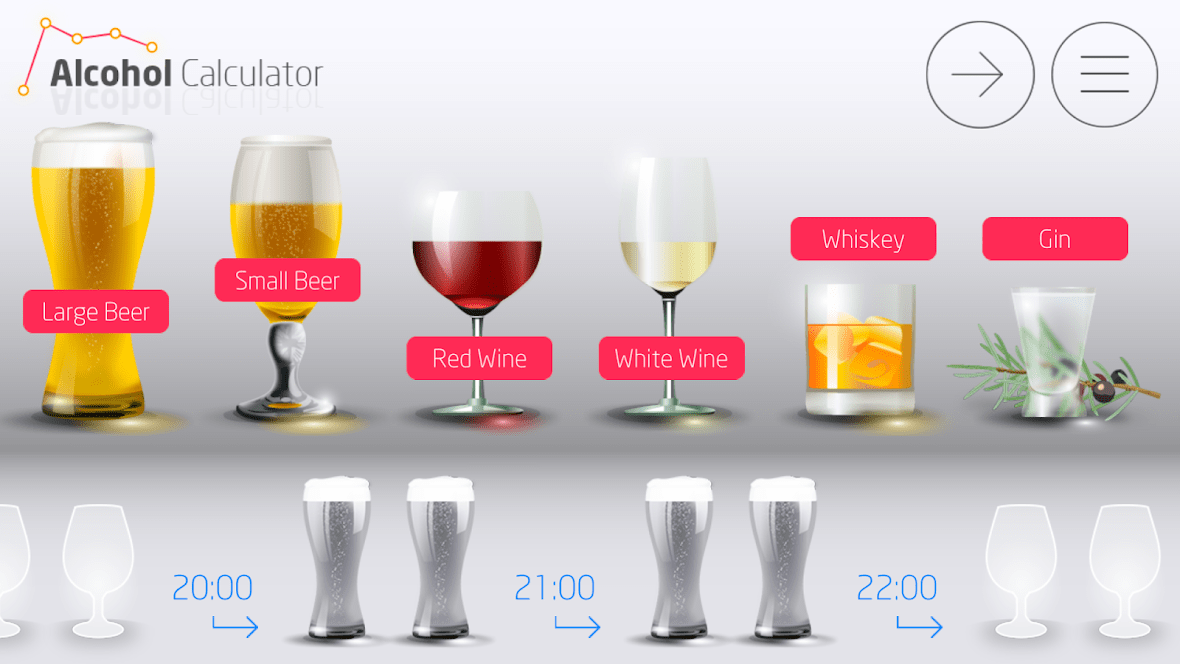
\includegraphics[width=1.1\textwidth]{./img/calculator.png}
      \caption{Blood Alcohol Calculator \cite{calculator} application}
      \label{calculator}
  \end{subfigure}\hfill
  \begin{subfigure}{0.38\textwidth}
      \centering
      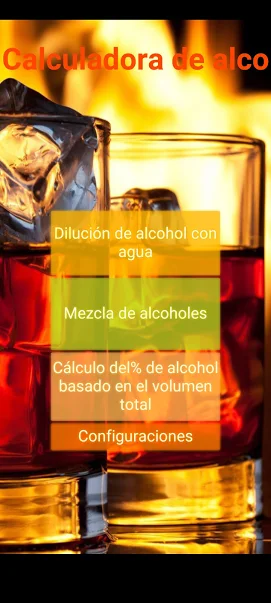
\includegraphics[width=0.4\textwidth]{./img/alcocal.png}
      \caption{Alco Calculator \cite{alcocal} application}
      \label{AlcoCalculator}
  \end{subfigure}
  \begin{subfigure}{0.3\textwidth}
      \centering
      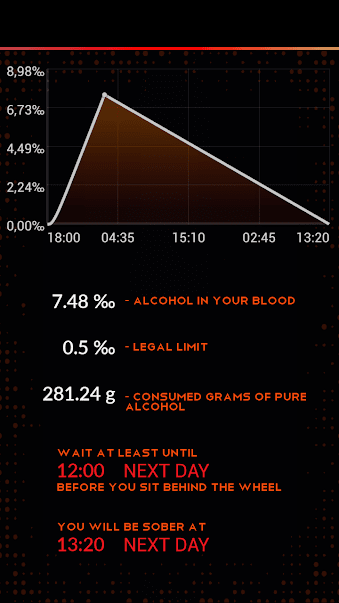
\includegraphics[width=0.65\textwidth]{./img/forfun.png}
      \caption{Alcohol test (for fun) \cite{forfun} application}
      \label{forfun}
  \end{subfigure}
  \caption{Screenshots of the different applications found in the Google Play \cite{googleplay}}
  \label{Screenshots}
\end{figure}

\newpage

  Drizly \cite{Drizly} is an application where the user can select different alcoholic beverages and get them delivered home. Alcotrack \cite{alcotrack} tracks alcohol consumption through self-report of alcoholic drinks. Alcoholcheck \cite{alcoholcheck} calculates blood alcohol content and an estimate of how long it will take you to reach zero level of alcohol in blood again after inserting gender, age, weight and consumed beverages.
  Alcofy \cite{Alcofy} is an application to add drinks in real time to see how drunk the user is and will be the next hours until they become sober. A limit can be set and the application will send a warning if the user is about to cross that limit. The estimated blood alcohol concentration is calculated based on a formula that has been studied and praised in scientific papers. Blood Alcohol Calculator \cite{alcoholcalculator} is an application to add weight, gender, drinks selected from a list of hundreds of built-in drinks or created/customized by the user and how long the user has been drinking to calculate the blood alcohol content of you and your friends. This shows the estimation of blood alcohol concentration and some possible side effects related to that blood alcohol range, as well as a detailed graph letting you know what your blood alcohol content will be over time. Simple Alcohol Unit Tracker \cite{saut} calculates the approximate blood alcohol concentration level based on the information about the user and their consumed alcoholic drinks. It has several options: calculation of blood alcohol concentration, reflex test, addition of new alcohol types and the setting of alcohol limits.
  Blood Alcohol Calculator \cite{calculator} calculates blood alcohol content and an estimate of how long it will take you to reach zero level of alcohol in blood again after inserting gender and consumed beverages. Alco Calculator \cite{alcocal} calculates the concentration of alcohol in a disolution (beverage or not). Alcohol test (for fun) \cite{forfun} is an application to add drinks and understand their alcohol consumption/drinking habits. A screenshot of each of these applications can be found in Figure \ref{Screenshots}.


\subsection{Scientific articles}

With respect to scientific articles found in Scopus \cite{scopus} and filtered as previously mentioned, different aspects have been taken into account:

\subsubsection{Countries from the affiliations}

Most of the affiliations are exclusively from USA \cite{Li2021,Mitchell2020297,Businelle2020,Suffoletto2020505,Killian201935,Willoughby2019496,Mariakakis2018,Suffoletto2018116,Leonard2017,Kinnamon2017}, but others were a colaboration of one or more countries out of the USA and a country from USA \cite{Sempionatto2019161,Bertholet2017285,Park201774}. Only three articles have affiliations exclusively from UK and those are \cite{Leightley2020,Garnett2019296,Leightley2018}. Australia participated in \cite{Poulton201835} and with Switzerland in \cite{Phan2020211}. Japan was the country of the affiliations of \cite{Wakana2019}, India was the country of affiliation of \cite{Chatterjee2018} and Denmark of \cite{Mellentin2017}. Table \ref{countries} summarizes the relation between countries and affiliations.

\begin{table}[h!]
  \centering
 \begin{tabular}{|| c | c ||}
 \hline
 \textbf{Country} & \textbf{Affiliations (out of 22)} \\ [0.5ex]
 \hline\hline
 USA & 13\\
 \hline
 UK & 4\\
 \hline
 Autralia & 3\\
 \hline
 Switzerland &  2\\
 \hline
 Brazil & 1\\
 \hline
 Canada & 1\\
 \hline
 Denmark & 1\\
 \hline
 Japan & 1\\
 \hline
 India & 1\\
 \hline
 South Korea & 1\\
 \hline
 Spain & 1\\
 \hline
 Thailand & 1\\ [0.5ex]
 \hline
\end{tabular}
\caption{Affiliations' countries of the different studies reviewed}
\label{countries}
\end{table}

\subsubsection{Sample size}

Most of the studies had a sample of less than 100 people summing all of the mentioned phases of the study, specifically 13 out of the 22 studies previously mentioned \cite{Li2021,Intarasirisawat2020,Mitchell2020297,Suffoletto2020505,Leightley2020,Killian201935,Sempionatto2019161,Leightley2018,Mariakakis2018,Suffoletto2018116,Leonard2017,Mellentin2017,Park201774}. Four of them \cite{Wakana2019,Garnett2019296,Chatterjee2018,Kinnamon2017} did not mention anything about the sample used in the study and the remaining five had samples between 120 and 671 subjects \cite{Phan2020211,Businelle2020,Willoughby2019496,Poulton201835,Bertholet2017285}. More information can be found in the Appendix \ref{appendix:matrix}.

\subsubsection{Diversity}

According to diversity, three different aspects were taken into account: age diversity, gender diversity and ethnic diversity.

Regarding age, eight of them \cite{Businelle2020,Wakana2019,Sempionatto2019161,Willoughby2019496,Garnett2019296,Chatterjee2018,Mellentin2017,Park201774} did not mention anything about the ages of the samples. Most of the rest have a wide age range, but four of them \cite{Phan2020211,Killian201935,Suffoletto2018116,Leonard2017} were specifically for young people therefore the age range was more limited.
Regarding gender, eight of them \cite{Businelle2020,Leightley2020,Wakana2019,Sempionatto2019161,Garnett2019296,Chatterjee2018,Mellentin2017,Park201774} did not mention anything about the gender and one mentioned diversity but did not mention ratios nor percentages. One had a 100\% of males with no specific reason \cite{Intarasirisawat2020} and another one had 100\% of females because the study wanted to study the impact of problematic alcohol drinking in female college students \cite{Leonard2017}. The rest of the studies were approximately half male and half female (some had up to 70\% one gender), except one \cite{Leightley2018}, that has almost 90\% male and only almost 10\% female.
Regarding ethnic, more than half of the studies, 15 out of 22 \cite{Li2021,Intarasirisawat2020,Phan2020211,Mitchell2020297,Leightley2020,Wakana2019,Sempionatto2019161,Willoughby2019496,Garnett2019296,Chatterjee2018,Leightley2018,Poulton201835}, did not mention anythihng about ethnic, four of them \cite{Businelle2020,Suffoletto2020505,Mariakakis2018,Bertholet2017285} mentioned diversity but did not specified proportions nor percentages and the rest were diverse. More information can be found in the Appendix \ref{appendix:matrix}.

\subsubsection{Applications}

Less than a fourth of the studies, 5 out of 22 \cite{Suffoletto2020505,Sempionatto2019161,Chatterjee2018,Kinnamon2017,Park201774}, did not use any smartphone application. One of the remaining studies \cite{Intarasirisawat2020} used pre-existing applications: Tetris, Fruit Ninja, and Unblock Puzzle, all three of them with some modifications to track important information; another 5 studies \cite{Phan2020211,Businelle2020,Wakana2019,Killian201935,Mellentin2017} used an application but did not mention the name and the rest used the following applications: Alcogait \cite{Li2021}, Ria Treatment Platform app \cite{Mitchell2020297}, Drinks:Ration \cite{Leightley2020}, DrunkSelfie \cite{Willoughby2019496}, Drink Less \cite{Garnett2019296}, InDEx (Information about Drinking for Ex-serving personnel) \cite{Leightley2018}, CNLab-A \cite{Poulton201835}, DUI (Drunk user interfaces) \cite{Mariakakis2018}, DrinkTRAC \cite{Suffoletto2018116}, Empatica \cite{Leonard2017} and Alcooquizz \cite{Bertholet2017285}.

\subsubsection{Device(s)}

Regarding devices, some of the studies used only smartphones \cite{Intarasirisawat2020,Phan2020211,Mitchell2020297,Suffoletto2020505,Wakana2019,Willoughby2019496,Garnett2019296,Chatterjee2018,Leightley2018,Poulton201835,Mariakakis2018,Suffoletto2018116,Bertholet2017285,Mellentin2017} and some others used smartphones and some kind of wearable \cite{Li2021,Businelle2020,Leightley2020,Killian201935,Leonard2017}. Only \cite{Park201774}, \cite{Sempionatto2019161} and \cite{Kinnamon2017} used only wearables (smart shoes, smart eyeglasses and electronic bracelet, respectively). Table \ref{devices} summarizes the devices and sensors used in the reviewed studies. More information can be found in the matrix attached in the Appendix \ref{appendix:matrix}.

\begin{longtable}[h!]{||p{.2\textwidth} | p{.25\textwidth} | p{.25\textwidth}| p{.25\textwidth}||}
\caption{Smartphone specifications  and measurements from smartphones used in the reviewed studies}
\label{devices}
\endfirsthead
\hline
\textbf{Study} & \textbf{Device(s)} & \textbf{Sensors} & \textbf{Measurements} \\
\hline
\hline
\endhead
\hline
\textbf{Study} & \textbf{Device(s)} & \textbf{Sensors} & \textbf{Measurements} \\
\hline
Li et al. (2021) \cite{Li2021} & Smartphone (Google Pixel XL) + wearable (LG Watch Sport) & \multirow{2}{=}{Accelerometer and gyroscope} & Gait changes \\ \cline{1-2} \cline{4-4}
Intarasirisawat et al. (2020) \cite{Intarasirisawat2020} & Smartphone (Samsung S6) &  & Device acceleration, rotational motion and touch-based features \\ \hline
Phan et al. (2020) \cite{Phan2020211} & Smartphone (Model not specified, Android OS) & Accelerometer, Bluetooth, WiFi, GPS, apps logs, camera & Location accuracy, speed, and GPS coordinates, network percentage; and mobility. human mobility, social context and person-person proximity \\ \hline
Mitchell et al. (2020) \cite{Mitchell2020297} & Smartphone (Model not specified and OS not specified) & Breathalyzer (External) & Alcohol in breath \\ \hline
Businelle et al. (2020) \cite{Businelle2020} & Smartphone (Samsung Galaxy J3 smartphone (or equivalent)) + wearable (SCRAM bracelet) & Geolocation & Longitude + latitude (geolocation), BAC  \\ \hline
Suffoletto et al. (2020) \cite{Suffoletto2020505} & Smartphone (Model not specified and OS not specified) & Accelerometer & Mean of acceleration signal, Variance of acceleration signal, Correlation of pairwise acceleration signals, Covariance of acceleration signal, Maximum difference of acceleration signal, Maximum difference of pairwise acceleration signals, Mean trend of acceleration signal of 0.1 second windows within the window, Windowed mean trend of acceleration signal of 0.1 second windows within the window, Variance trend of acceleration signal, Windowed variance trend of acceleration signal \\ \hline
Leightley et al. (2020) \cite{Leightley2020} & Smartphone (Model not specified, Android and iOS OS) + wearable (not specified) & GPS, push notifications & Location, heart rate, distance travelled, activities, height, and weight \\ \hline
Wakana \& Yamada (2019) \cite{Wakana2019} & Smartphone (Model not specified and OS not specified) & Breathalyzer (External) & Breath Alcohol Concentration (BrAC) \\ \hline
Killian et al. (2019) \cite{Killian201935} & Smartphone (Model not specified, Android and iOS OS) wearable (SCRAM bracelet) & Accelerometer & Acceleration/movement and TAC (transdermal alcohol content) \\ \hline
Sempionatto et al. (2019) \cite{Sempionatto2019161} & Wearable (smart glasses) & Alcohol biosensor and amperometric sensor & Alcohol and Glucose in tears \\ \hline
Willoughby et al. (2019) \cite{Willoughby2019496} & Smartphone (Model not specified, Android OS) & Camera & Face Detection, Locating Facial Landmarks, Aligning Faces using Landmarks, Landmark positions, Landmark vectors, Landmark lines, Detecting facial lines and wrinkles using Canny Edge detection and the Hough transform, Forehead redness, Smiles, Lips and Eyes \\ \hline
Garnett et al. (2019) \cite{Garnett2019296} & Smartphone (Model not specified, iOS OS) & None & ABV (alcohol by volume), size, quantity and price. Mood, productivity, clarity and sleep quality. Calorie intake, spend on alcohol, and how mood, productivity, clarity and sleep quality are affected by heavy drinking. \\ \hline
Chatterjee, Isha and Sharma (2018) \cite{Chatterjee2018} & Smartphone (Model not specified and OS not specified) & Camera & Video of the person \\ \hline
Leightley et al. (2018) \cite{Leightley2018} & \multirow{2}{=}{Smartphone (Model not specified, Android and iOS OS)} & \multirow{2}{=}{None} & Amount of alcohol consumed, how and when \\ \cline{1-1} \cline{4-4}
Poulton et al. (2018) \cite{Poulton201835} & &  & Quantity, frequency, type of alcohol, start and finish times \\ \hline
Mariakakis et al. (2018) \cite{Mariakakis2018} & Smartphone (Third-generation Moto G smartphone) & Touchscreen, accelerometer, and gyroscope, flash and camera & How correctly they write and if they correct or not the mistakes, also how the subject maintain the balance, heart rate \\ \hline
Suffoletto et al. (2018) \cite{Suffoletto2018116} & Smartphone (Model not specified, iOS OS) & Accelerometer, gyroscope and magnetometer & Real, dynamic and static acceleration, angular velocity, attitude of the device \\ \hline
Leonard et al. (2017) \cite{Leonard2017} & Smartphone (Model not specified, Android OS) wearable (Empatica E4 wrist band) & Electrodermal activity (EDA), accelerometer and temperature sensor & Real-time EDA, movement, temperature, heart rate \\ \hline
Bertholet et al. (2017) \cite{Bertholet2017285} & Smartphone (Model not specified, Android and iOS OS) & None & Quantity and frequency of alcohol consumption \\ \hline
Kinnamon et al. (2017) \cite{Kinnamon2017} & Wearable (Electronic Bracelet for Monitoring of Alcohol Lifestyle) & Immunoassay based EtG biosensor & Ethyl glucuronide (EtG) in sweat \\ \hline
Mellentin et al. (2017) \cite{Mellentin2017} & Smartphone(Model not specified, Android OS) & App logs & Real-time measures of cue-induced cravings. \\ \hline
Park et al. (2017) \cite{Park201774} & Wearable (smart shoes) & Array of pressure sensors & Pressure of the feet when walking \\ \hline
\end{longtable}


As shown in Table \ref{devices}, more than a fifth are multiplatform, available for both Android and iOS, almost a fifth works for Android and almost a fifth does not specify the operative system. Some of them have specific models, like Samsung S6, Samsung Galaxy J3 (or equivalent), Third-generation Moto G and Google Pixel XL. Table \ref{smartphonespecifications} sums up the different devices used along the studies. Not a lot of wearables are used. Some of them are SCRAM bracelet, Empatica E4 wrist band and LG Watch Sport. Table \ref{wearables} summarizes the different wearables used in the reviewed studies.

\begin{table}[h!]
  \centering
 \begin{tabular}{||c | c ||}
 \hline
 \textbf{Smartphone specifications} & \textbf{Studies (out of 22)} \\ [0.5ex]
 \hline \hline
  Model not specified, Android and iOS &  5\\
  \hline
 Model and OS not specified & 4\\
 \hline
 Model not specified, Android OS & 4\\
 \hline
 Model not specified, iOS OS & 2\\
 \hline
 Samsung S6 & 1\\
 \hline
 Samsung Galaxy J3 (or equivalent) & 1\\
 \hline
 Third-generation Moto G & 1\\
 \hline
 Google Pixel XL & 1\\[0.5ex]
 \hline
\end{tabular}
\caption{Smartphone specifications from smartphones used in the reviewed studies}
\label{smartphonespecifications}
\end{table}

\begin{table}[h!]
  \centering
 \begin{tabular}{||c | c ||}
 \hline
 \textbf{Wearables} & \textbf{Studies (out of 22)} \\ [0.5ex]
 \hline\hline
 SCRAM bracelet & 2\\
 \hline
 LG Watch Sport & 1\\
 \hline
 Not specified & 1\\
 \hline
 Empatica E4 wrist band &  1\\
 \hline
 Electronic Bracelet for Monitoring of Alcohol Lifestyle & 1\\[0.5ex]
 \hline
\end{tabular}
\caption{Wearables used in the reviewed studies}
\label{wearables}
\end{table}

\subsubsection{Sensors}

The most used sensors are accelerometer and gyroscope, but also geolocation, camera and temperature sensors. Some of the studies do not mention the use of any kind of sensors \cite{Garnett2019296,Leightley2018,Poulton201835,Bertholet2017285}. Table \ref{sensors} summarizes the use of sensors. More  information can be found in table \ref{devices} and in the Appendix \ref{appendix:matrix}.

\begin{table}[h!]
  \centering
 \begin{tabular}{||c | c ||}
 \hline
 \textbf{Sensors} & \textbf{Studies (out of 22)} \\ [0.5ex]
 \hline\hline
 Accelerometer & 8\\
 \hline
 Gyroscope & 4\\
 \hline
 Camera & 3\\
 \hline
 Application logs &  2\\
 \hline
 Geolocation &  2\\
 \hline
 Breathalyzer & 2\\
 \hline
 Bluetooh & 1\\
 \hline
 WiFi &  1\\
 \hline
 Flash & 1\\
 \hline
 Push notifications & 1\\
 \hline
 Alcohol biosensor & 1\\
 \hline
 Amperometric sensor & 1\\
 \hline
 Touchscreen &  1\\
 \hline
 Magnetometer & 1\\
 \hline
 Electrodermal activity (EDA) & 1\\
 \hline
 Temperature & 1\\
 \hline
 Immunoassay based EtG biosensor &  1\\
 \hline
 Pressure &  1\\
 \hline
 None & 4\\[0.5ex]
 \hline
\end{tabular}
\caption{Sensors \cite{Businelle2020} used in the reviewed studies}
\label{sensors}
\end{table}


\subsubsection{Mobile self-report}

Almost half of the studies (10 out of 22) use mobile self-report as an information collector. Of those 10 studies, in 8 of them \cite{Phan2020211,Businelle2020,Leightley2020,Garnett2019296,Leightley2018,Poulton201835,Suffoletto2018116,Bertholet2017285} the user added information about alcohol consumption: type of alcohol, amount of beverage, time elapsed when drinking...; one \cite{Leonard2017} asked for information about feelings when a notification popped up and the last one \cite{Mellentin2017} was about cravings when staring at alcoholic beverages. More information can be found in the Appendix \ref{appendix:matrix}.

\subsubsection{Measurements}

Most of the measurements taken are physical ones, related to location and motion like acceleration and movement, but also measurements related to drinking like quantity, frequency, type of alcohol and start and finish times when drinking. Also alcohol in blood, breath and transdermal are meassured. Some studies use videos \cite{Chatterjee2018} or selfies \cite{Willoughby2019496} of the user. More information can be found in table \ref{devices} and in the Appendix \ref{appendix:matrix}.

\subsubsection{Methods}

Table \ref{methods} summarizes the methods to proccess the previously mentioned data gathered from the sensors and the output obtained with this proccesses.

\begin{longtable}{||p{.2\textwidth} | p{.25\textwidth} | p{.25\textwidth} | p{.25\textwidth}||}
\caption{Methods to proccess measurements and outputs from them in the reviewed studies}
\label{methods}
\endfirsthead
\hline
\textbf{Study} & \textbf{Methods} & \textbf{Output} & \textbf{Drawbacks} \\
\hline
\hline
%
\endhead
\hline
\hline
\textbf{Study} & \textbf{Methods} & \textbf{Output} & \textbf{Drawbacks} \\ \hline
Li et al. (2021) \cite{Li2021} & Machine Learning & Warning while drinking/on the way to the car & Possible bias in layer normalization and methods towards certain subjects \\ \hline
Intarasirisawat et al. (2020) \cite{Intarasirisawat2020} & Machine Learning & Visualization & No gender diversity. Exclusion of people with different conditions. Small sample of study/control. \\ \hline
(Phan, Labhart, Muralidhar \& Gatica-Perez, 2020) \cite{Phan2020211} & Machine learning & Classifiication of the consumption: heavy or non-heavy drinking & No assurance data is correctly inserted, bias in self-report \\ \hline
Mitchell et al. (2020) \cite{Mitchell2020297} & Statistics & Models for the relationship between BAC and time & No control group. Patients were highly motivated. Approximately 46\% of data for the BAC readings were missing.\\ \hline
Businelle et al. (2020) \cite{Businelle2020} & Others & Text messages to in-the-moment distraction, reframing, immediate help-seeking, planning, and other tools to reduce craving. & The intervention app may not be applicable to those with low literacy and cognitive impairment. EMA or SCRAM monitoring may have independent effects on drinking. Self-monitoring can lead to changes in drinking, even without an “intended” intervention. \\ \hline
Suffoletto et al. (2020) \cite{Suffoletto2020505} & Machine Learning & Models, regressions and predictions of excessive alcohol consumption & Small sample size, the use of a cohort that largely drinks below risky levels, and controlled setting of data measurement. It did not examine whether gait-related features discriminate lower levels of drinking. It placed the smartphone on the lower back, which may not represent where individuals keep their phones in natural environments. Did not find that population-based models were accurate in predicting intoxication. \\ \hline
Leightley et al. (2020) \cite{Leightley2020} & Statistics & Push notifications/ SMSs to warn/inform the subject & \multirow{2}{*}{-} \\ \cline{1-3}
Wakana \& Yamada (2019) \cite{Wakana2019} & Others & Estimated BrAC and detection of saturated water vapor and the metabolites &  \\ \hline
Killian et al. (2019) \cite{Killian201935} & Machine Learning & Clasification of sobriety every 10 seconds. & Low control of the phone placement, low accuracy of accelerometer, classifiers had a higher accuracy for sober data than intoxicated data and that the variance of the best classifier was high for intoxicated subjects.\\ \hline
Sempionatto et al. (2019) \cite{Sempionatto2019161} & Others & Estimation of glucose and alcohol in blood & Small sample size. small sample volumes of the extracted tears, ease of sample evaporation during collection (particularly in sampling ethanol), potential composition variations between individuals and dependence on the sampling method. \\ \hline
Willoughby et al. (2019) \cite{Willoughby2019496} & Machine Learning & Classification of images: drunk or sober & Limited Dataset, Coarse Classification, Smartphone Internet Access Requirement and Comprehensive evaluation of DrunkSelfie app by users \\ \hline
Garnett et al. (2019) \cite{Garnett2019296} & Basic statistics & Feedback and graphics about goals. & \multirow{2}{*}{-} \\ \cline{1-3}
Chatterjee, Isha and Sharma (2018) \cite{Chatterjee2018} & Computer vision techniques of facial landmark detection and motion detection & Alert sound and location notification if the subject is drunk or drowsy &  \\ \hline
Leightley et al. (2018) \cite{Leightley2018} & Basic statistics & SMS with information and warnings, statistics of usage of the application and visualization of data from the reports & No assurance data is correctly inserted, not a long-term analysis, sample is very small, possible selection bias of the participants \\ \hline
Poulton et al. (2018) \cite{Poulton201835} & Statistics & Average daily and weekly consumption, hourly rate of consumption each day, days of consumption, total drinks and days in which 4 or 6 or 8 or (and so forth) more drinks were drunk & Limited alcohol options, no assurance data is correctly added \\ \hline
Mariakakis et al. (2018) \cite{Mariakakis2018} & Machine learning & Estimation of BAL (Blood alcohol level) & It doesn't meassure BAL directly \\ \hline
Suffoletto et al. (2018) \cite{Suffoletto2018116} & Machine Learning & Accurate prediction of blood alcohol concentration during drinking episodes & Sample is very small. Missing gait task data. Participants were paid to complete tasks, which likely artificially inflated completion rates. App was made only for iOS devices. Possible wrong insertion of alcohol drinks. \\ \hline
Leonard et al. (2017) \cite{Leonard2017} & Psycological & Analysis of the emotion + context, sum of use of screen with the app, amount of reports & Sample is very small. The form of the band was not accurate and the participants often forgot to charge it. The connection was not great and some alerts were inopportune \\ \hline
Bertholet et al. (2017) \cite{Bertholet2017285} & Statistics & Statistics about alcohol consumption habits & The uncontrolled design does not allow us to infer causation, further study is needed to evaluate the application's efficacy. Assessment of alcohol consumption relied on self-report, therefore social desirability bias or recall bias are possible. Assessment of app use also relied on self-report. \\ \hline
\pagebreak
Kinnamon et al. (2017) \cite{Kinnamon2017} & Electrochemical & Visualization of graphs with information about voltage, intensity and EtG concentration & \multirow{3}{*}{-} \\ \cline{1-3}
Mellentin et al. (2017) \cite{Mellentin2017} & Basic statistics & Measures and graphs to keep track of their training activities and potential advances in controlling cue reactivity &  \\ \cline{1-3}
Park et al. (2017) \cite{Park201774} & Machine Learning & A pressure distribution map and classification of the gait &  \\ \hline
\end{longtable}

Most of the studies use machile learning techniques like Logistic Regression (LR), Linear Support Vector Machine (LSVM), Random Forest (RF), Bi-directional Long Short Term Memory (Bi-LSTM) and Convolutional Neural Network (CNN), in addition to Cross-Validation (CV).
Statistics like average, median, summations, t-tests and chi-square tests are also used by some studies.
\cite{Kinnamon2017} uses square wave voltammetry (SWV), an electrochemical methods, \cite{Chatterjee2018} uses computer vision techniques of facial landmark detection and motion detection.
Others use techniques such as tears estimulation and alcohol and glucose detection in tears like \cite{Sempionatto2019161}, questionnaires for developing + 'real time' drinking algorithm for testing like \cite{Businelle2020} or a calculation algorithm based on a differential evolutional method like \cite{Wakana2019}. The summary of the usage of these methods can be seen in table \ref{studymethods}.

\begin{table}[h!]
  \centering
 \begin{tabular}{||c | c ||}
 \hline
 Method & Studies (out of 22) \\ [0.5ex]
 \hline\hline
 Machine Learning & 9\\
 \hline
 Statistics & 7\\
 \hline
 Computer vision techniques & 1\\
 \hline
 Psycological &  1\\
 \hline
 Electrochemical &  1\\
 \hline
 Others & 3\\[0.5ex]
 \hline
\end{tabular}
\caption{Methods used in the studies}
\label{studymethods}
\end{table}

\subsubsection{Output}

There is a wide range of outputs, from visualization to classification, but also notifications, models for the relationship between drinking and time estimations of alcohol in blood. More information can be found in Table \ref{methods} and in the Appendix \ref{appendix:matrix}.

\subsubsection{Drawbacks}

The most common drawbacks are the small sample size and the lack of control of some variables, like low control of the phone placement, low accuracy of accelerometer or no assurance data is correctly inserted. More information can be found in Table \ref{methods} and in the Appendix \ref{appendix:matrix}.

\subsubsection{Conflicts of interest}

None of the above mentioned articles had any conflicts of interest but these four:

\begin{itemize}
  \item John Mendelson is the owner of Ria Health. The remaining authors have nothing to disclose \cite{Mitchell2020297}.
  \item MB is an inventor of the Insight mHealth Platform and receives royalties related to use of this platform \cite{Businelle2020}.
  \item NTF sits on the Independent Group Advising on the Release of Data at NHS Digital. NTF is also a trustee of a military-related charity. AS is a full-time member of the Armed Forces seconded to King’s College London. DM and CW are employed by Combat Stress, a national charity in the United Kingdom that provides clinical mental health services to veterans \cite{Leightley2020}.
  \item J.B. has received unrestricted research funding from Pfizer related to smoking cessation. R.W. has received research funding and undertaken consultancy for companies that manufacture smoking cessation medications. R.W. and S.M. are advisers to the National Centre for Smoking Cessation and Training. S.M. is Director of the UCL Centre for Behaviour Change \cite{Garnett2019296}.
\end{itemize}

\newpage

%\input{methodology.tex}
\newpage
\section{Design}
\label{design}

\subsection{Horizontal Gaze Nystagmus}

Due to the effects of alcohol consumption in the Nystagmus movements, the US police use horizontal gaze Nystagmus as a test, additionally to two others standarized tests (walk and turn and one-leg-stand), to check whether to arrest someone (if they are drunk) or to let them free (if they are sober).The National Highway Traffic Safety Administration of United States wrote a complete guide about the science and usage of Horizontal Gaze Nystagmus for judges, prosecutors and law enforcement \cite{NystagmusTest} in which can be found a deep explanation of the test's performance. Figure \ref{nystagmus} summarizes the parameters the police officer would check if it was an in-person test.

\begin{figure}[H]
    \centering
    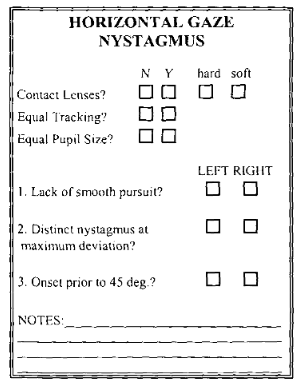
\includegraphics[width=0.5\textwidth]{./img/nystagmus.png}
    \caption{Parameters check by the police officers. Reprinted from \cite{NystagmusTest}.}
    \label{nystagmus}
\end{figure}

To perform this test, the police officer will firstly ask the subject whether they wear lenses and if the answer is positive, whether they are hard or soft. Secondly, they will check that both eyes have an equal tracking of the object, such as a pen or the tip of a penlight, used for the test and the equality of both pupils' size. The use or not of contact lenses, hard or soft, do not affect the test in any way, contrary to some concerns. The lack of equal tracking or equal pupil size may indicate blindness in one eye, a glass eye, a medical disorder or an injury. If the subject exhibits these characteristics, the officer should discontinue the test and may need to seek medical assistance for the individual if a medical disorder or injury appears to exist. After these checks, the test starts with three different clues (each of the subtests performed to check the gaze): lack of smooth pursuit, distinct nystagmus at maximum deviation and onset prior to 45 degrees. These three clues are performed asking the suspect to follow the object, placed 12 to 15 inches away (approximately 30-40cm), with only their eyes, both to the left and the right sides, summing up six clues in total. Failing at least two out of this six clues is enough to fail the test.

The first two clues, left and right lack of smooth pursuit, is obtained by moving the object slowly but steadily from the center of the subject's face towards the left and the right ears respectively. The left and right distinct nystagmus at maximum deviation is obtained by, starting again from the center of the suspect's face, moving the object toward the left and right ears respectively, bringing the eye as far over as possible, and holding the object there for four seconds to ensure that quick movement of the object did not possibly cause the nystagmus. The left and right onset prior to 45 degrees is done by moving the object at a speed that would take about four seconds for the object to reach the edge of the suspect's left and right shoulder respectively. The officer notes this clue if the point or angle at which the eye begins to display nystagmus is before the object reaches forty-five degrees from the center of the suspect's face. This test can be seen in a YouTube \cite{YouTube} video called 'Horizontal Gaze Nystagmus: The Truth is in the Eyes' \cite{YouTubeVideo}.

\subsection{Requirements}

The MoSCoW prioritization method \cite{moscow} is used to classify the requirements of this project. MoSCoW is an acronym for "Must have, Should have, Could have and Won’t have", categories in which requirements are divided.

\begin{itemize}
  \item \textbf{Must have requirements:} They are critical for the success of the project.
    \begin{itemize}
      \item The mobile application must be cross-platform.
      \item The user must be able to record videos.
      \item The application must determine whether it is safe for the user to drive or not.
      \item The application must show instructions to the user to perform the different clues.
      \item The system must support modularity and scalability.
    \end{itemize}
  \item \textbf{Should have requirements:} These are important requirements, but not necessary for the system release.
    \begin{itemize}
      \item The system should store the tests and their clues for further research.
      \item The application must have a 'Terms and Conditions' section explaining the usage and treatment of their data.
      \item The application should show a preview of the recorded video.
      \item The application should have a 'Help' section explaining how the test works.
    \end{itemize}
  \item \textbf{Could have requirements:} Desirable requirements that could improve user’s experience or satisfaction. They will be included if there is time at the end of the development.
    \begin{itemize}
      \item The application could show a loading screen when the videos are being proccessed.
      \item The user could give feedback about their experience and accordance with the result of the test.
      \item The system could provide a dashboard to analyze test results statistics.
      \item The application could provide information about alcohol consumption and the hazzards of driving after drinking.
      \item The application could allow the user to order a taxi if the test fails.
    \end{itemize}
  \item \textbf{Won't have requirements:} They are inappropiate or the least important ones, so they are not included in the project.
    \begin{itemize}
      \item The user won't be able to log into the application with any social sign-in (i.e. Google, Facebook).
      \item The application won't check the pupil size nor the smooth gaze.
      \item The stored user data won't be sensitive.
    \end{itemize}
\end{itemize}

\subsection{Architecture}

In the designed system there are two subsystems: the mobile application and a server to host a database and a the backend to proccess data sent from the application. The user interacts with the smarphone sending videos and receiving instructions and feedback from it. The smartphone firstly sends a request to the endpoint to initialize the test and the first clue. Then, it calls the backend to finish the current clue, update the test's end timestamp and create the next clue database entry. For this purpose, it calls each of the endpoints named after each of the clues. The API can perform the create and update operations to the tests and clues on the database, and the database returns an ACK. Figure \ref{architecture} shows the previously explained architecture of the system.

\begin{figure}[H]
    \centering
    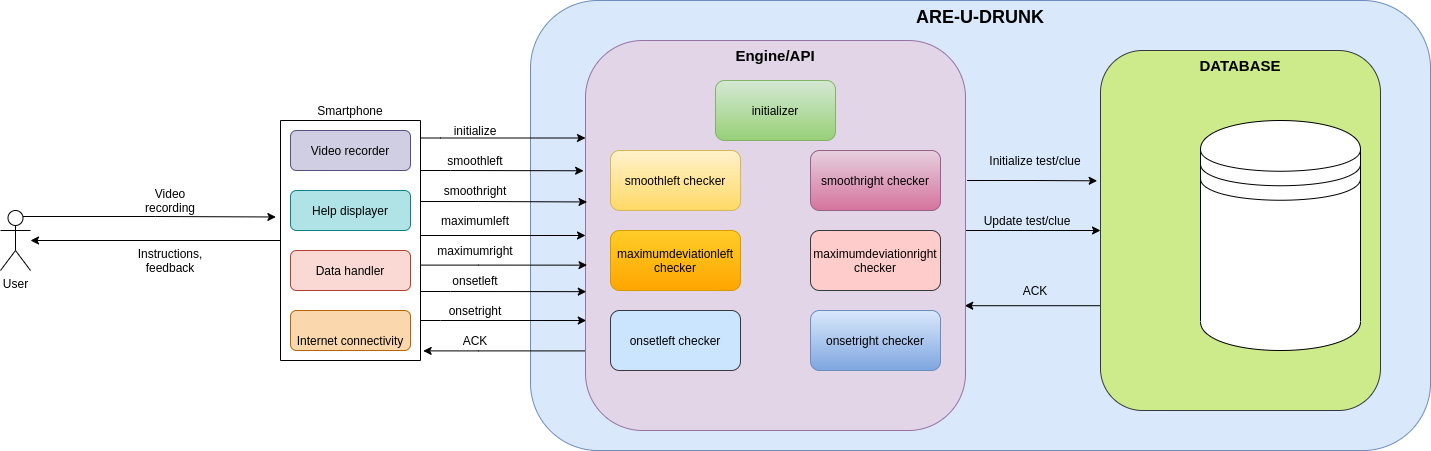
\includegraphics[angle=90, height=23cm,keepaspectratio]{./img/Architecture.png}
    \caption{Architecture of the system}
    \label{architecture}
\end{figure}



\subsubsection{Mobile application}

When designing the mobile application, the test prerequisites (pupil size and smooth gaze) are not considered because of the limitations of the current technology: the pupil size is very difficult to calculate because it depends on the distance to the camera and the angle of the face with respect to the phone. For this reason, the prerequisites are assumed to be correct and the mobile application is desinged as figure \ref{viewflow} shows.

\begin{figure}[H]
    \centering
    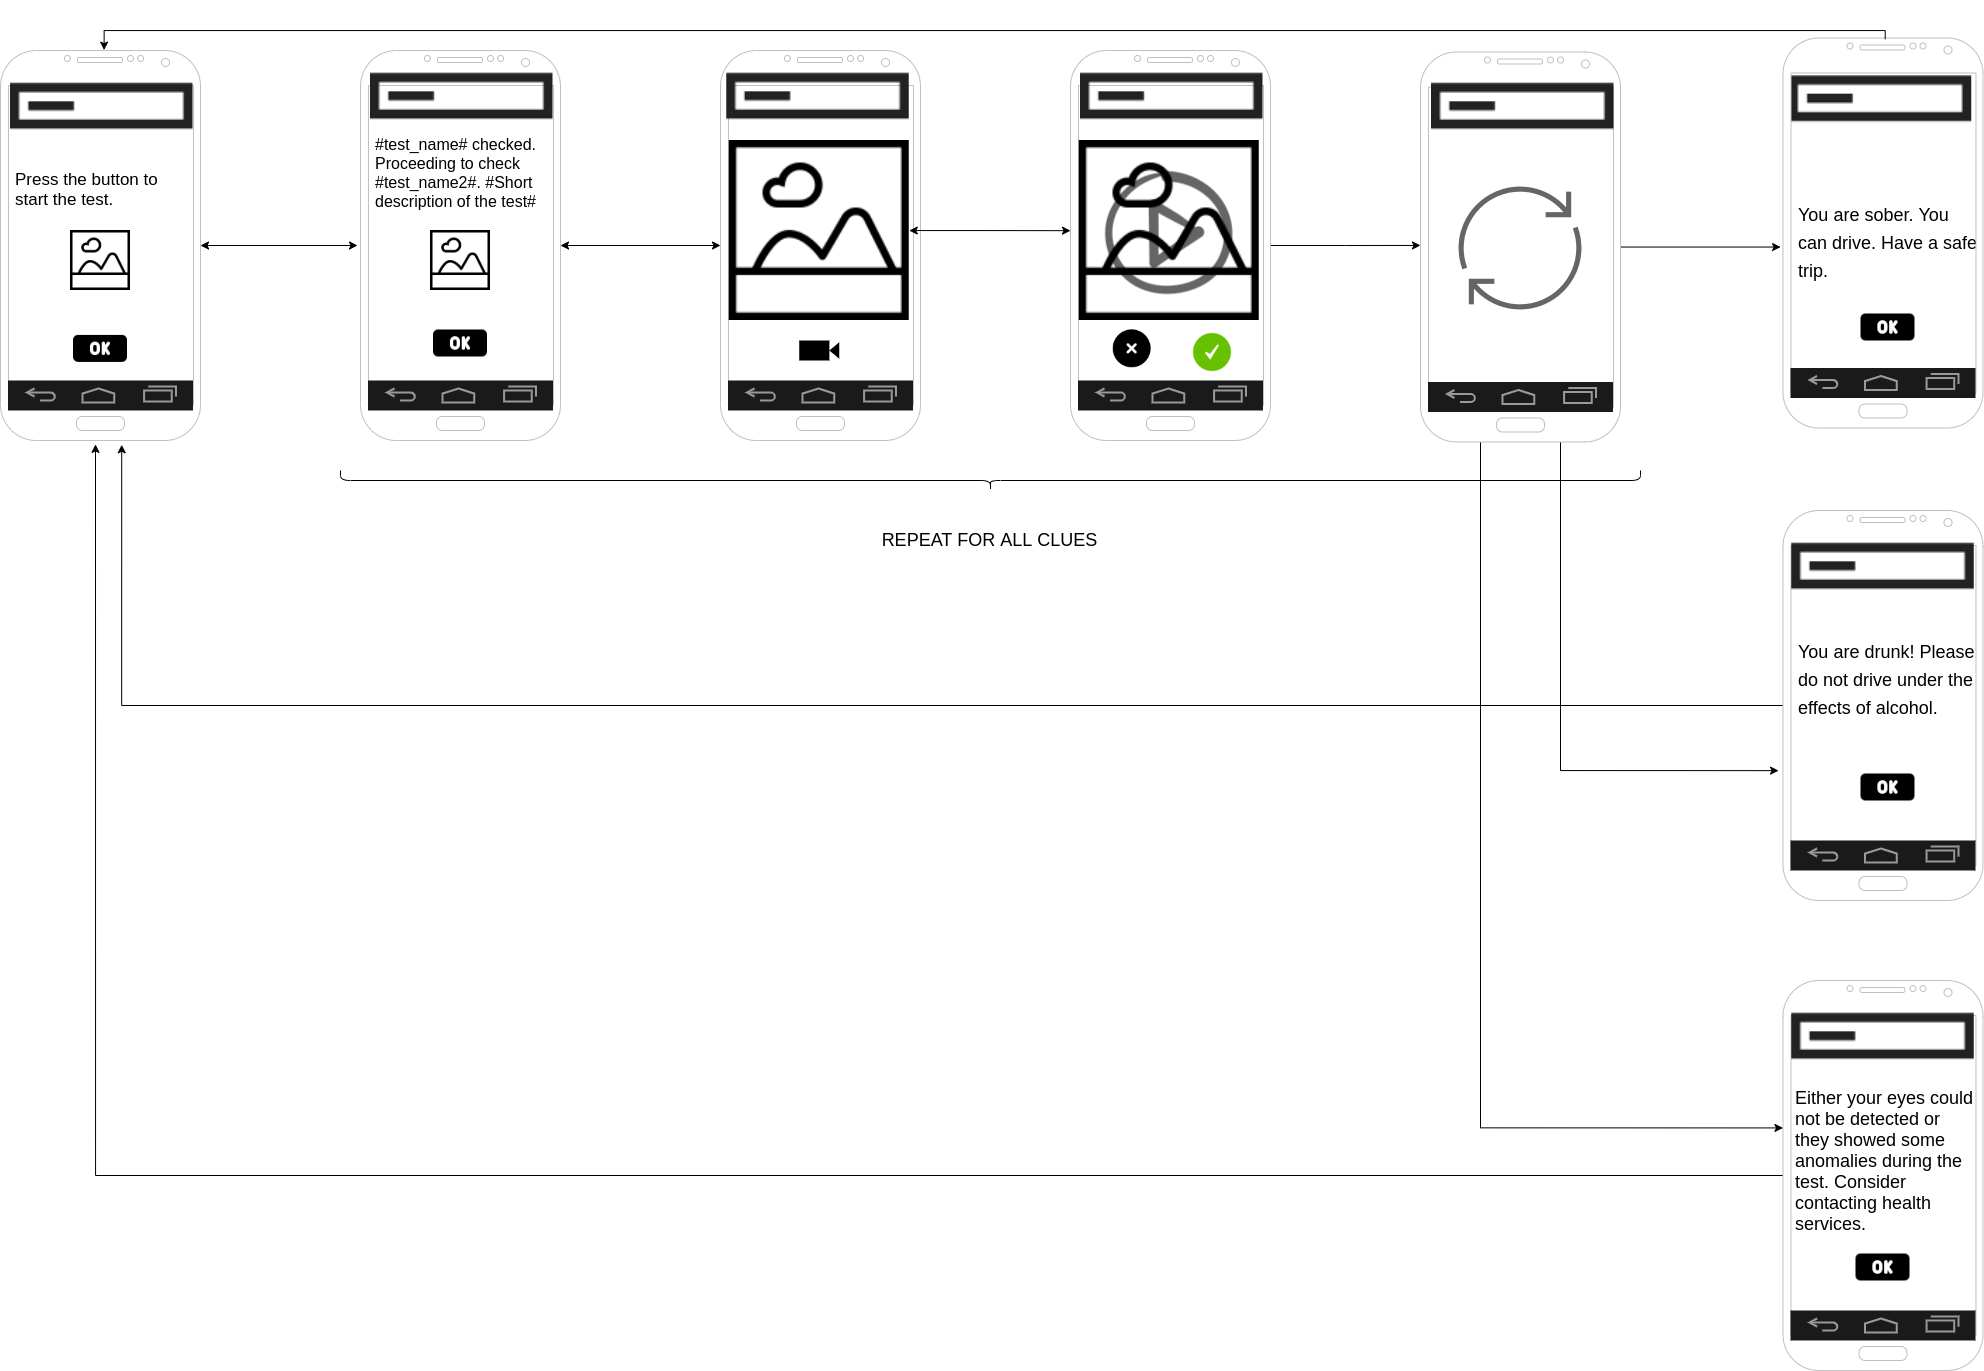
\includegraphics[angle=90, width=\textwidth]{./img/viewflow.png}
    \caption{View flow of the application}
    \label{viewflow}
\end{figure}

The application starts with a screen in which the user is informed that the test will start as soon as they click the button. Then, the user is redirected to a screen with the instructions for the clue. When pressing the camera button, the application displays a camera preview in which the user can record a video and then is redirected to a video preview where the user can confirm or discard the recorded video. In case the video is discarded, the user can record another video until the user confirms the video. This is repeated for all of the clues while less than two clues fail. If five or more clues are correct, the user is finally redirected to a screen with a success message. If two clues fail, the test stops and the user is redirected to a screen with a message encouraging the user not to drive. If the eyes are not detected in any of the clues, the test stops and the user is redirected to a screen with a message encouraging the user to reach for professional help.

Figure \ref{flowchart} shows how the user interacts with the application and the application with the server.

\begin{figure}[H]
    \centering
    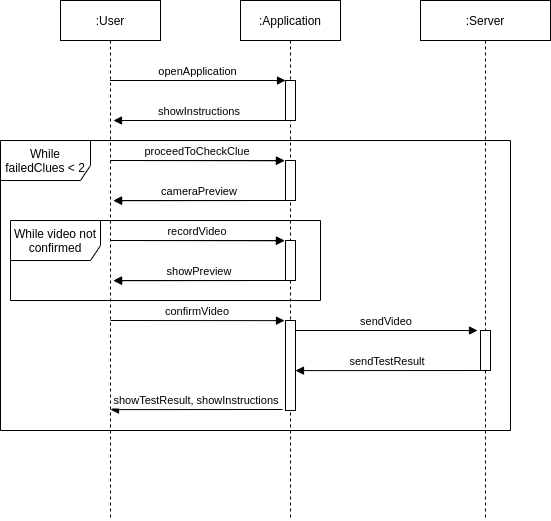
\includegraphics[width=0.95\textwidth]{./img/flowchart.png}
    \caption{View flow of the application}
    \label{flowchart}
\end{figure}

\subsubsection{Server}

The server consists on two modules: the database and an REST API that interacts with the database and the application.

The database contains relevant data about the tests and the clues, like:

\begin{itemize}
  \item Start and end timestamps of the tests.
  \item An unique user identifier.
  \item The URL where the video is stored.
  \item The type of clue.
  \item The result of the test and each of the clues.
\end{itemize}

The API receives the clues' data (videos) sent from the application. Each of the clues call their own endpoint that proccesses them to determine whether the clue is passed or failed, returns the results to the mobile application and finally creates the corresponding entries in the database, storing the video in a folder in the server. This interaction is shown in Figure \ref{architecture}.

\newpage
\section{Implementation}
\label{implementation}

When implementing this mobile application, the following technologies are being used:

\begin{itemize}
  \item \textbf{Flutter 2.2.1} \cite{Flutter}: Flutter is an open-source UI software development kit created by Google. It is used to develop cross platform applications and the web from a single codebase. Flutter was used instead of previously settled technologies such as Java \cite{Java}, Swift \cite{Swift} or Kotlin \cite{Kotlin} due to the first funtional requirement: cross platform compatibility.
  \item \textbf{Android Studio 4.2} \cite{AndroidStudio}: Android Studio is the official integrated development environment (IDE) for Google's Android \cite{Android} operating system. Android Studio is used due to the great compatibility with Flutter.
  \item \textbf{Python 3.8.5} \cite{Python}: Python is an interpreted high-level general-purpose programming language. Python is used due to its community and wide documentation about iamge and video documentation.
  \begin{itemize}
    \item \textbf{Flask 2.0.1} \cite{Flask}: Flask is a micro web framework written in Python. Flask is used due to its ease of use to create APIs. This API is used to integrate the application and Python code.
    \item \textbf{Gunicorn 20.1.0} \cite{Gunicorn}: Gunicorn is a Python WSGI HTTP Server for UNIX. It is used to deploy the API.
    \item \textbf{sqlalchemy 1.4.20} \cite{sqlalchemy}: SQLAlchemy is the Python SQL toolkit and Object Relational Mapper. It is used to design and manage the database.
    \item \textbf{psycopg2 2.9.1} \cite{psycopg2}: Psycopg is the most popular PostgreSQL database adapter for the Python programming language.
  \end{itemize}
  \item \textbf{PostgreSQL 12.7} \cite{postgres}: PostgreSQL is a powerful, open source object-relational database. It is the chosen database to store the data from the analyzed tests and clues.
  \item \textbf{Docker 20.10.7} \cite{Docker}: Docker is a set of platform as a service (PaaS) products that use OS-level virtualization to deliver software in packages called containers. Docker is used due to its portability and scalability.
  \item \textbf{pgAdmin 5.4} \cite{pgAdmin}: pgAdmin is the most popular and feature rich Open Source administration and development platform for PostgreSQL, the most advanced Open Source database in the world.
\end{itemize}

When integrating Python and Flutter, two Flutter plugins were considered:

\begin{itemize}
  \item \textbf{starflut} \cite{starflut}: This plugin was discarded due to the lack of good documentation, since this would make development, maintenance and addition of functionality difficult.
  \item \textbf{chaquopy} \cite{chaquopy}: This plugin is only available for Android \cite{Android}, discarding it with no further research due to the first funtional requirement: cross platform compatibility.
\end{itemize}
\subsection{Mobile application}

For the implementation of the application, four different views have been developed: an info page, a camera preview page, a video preview page and a result page. All of these base pages are parents to the different application screens. This avoids repeating code for similar views. Figure \ref{startpage} shows the Start Page of the application.

\begin{figure}[H]
  \centering
  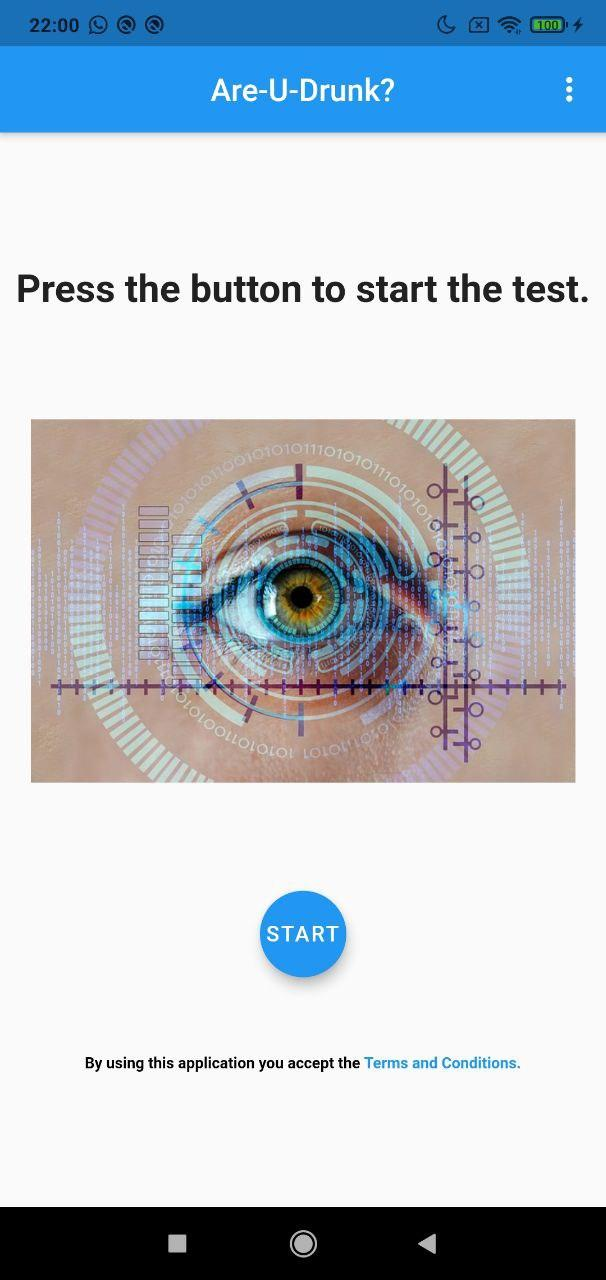
\includegraphics[width=0.25\textwidth]{./img/startpage.jpg}
  \caption{Start Page}
  \label{startpage}
\end{figure}

Code listing \ref{popupcode} shows how the Popup menu button works and listing \ref{termsandconds} how the link to the Terms and Conditions document is created. Listing \ref{startbutton} shows how the button is created and how it calls the backend to initialize the test and the first clue when it is pressed.


\begin{lstlisting}[language=flutter, basicstyle=\small, caption={Popup menu button code}, captionpos=b, label={popupcode}]
PopupMenuButton(
              itemBuilder: (BuildContext bc) => [
                PopupMenuItem(child: Text("Help"), value: "/help"),
              ],
              onSelected: (route) {
                Navigator.push(
                    context,
                    MaterialPageRoute(
                    builder: (context) => HelpPage()));
              },
            )
\end{lstlisting}


\begin{lstlisting}[language=flutter, basicstyle=\small, caption={Terms and Conditions document link}, captionpos=b, label={termsandconds}]
RichText(
  text: new TextSpan(
    children:[
     new TextSpan(
       text:"By using this application you accept the ",
       style: TextStyle(color: Colors.black, fontSize: 10, fontWeight: FontWeight.bold),
     ),
      TextSpan(
        text: "Terms and Conditions.",
        style: new TextStyle(color: Colors.blue, fontSize: 10,fontWeight: FontWeight.bold),
        recognizer: new TapGestureRecognizer()
        ..onTap = () async {
          final url = '<TCs URL>';
          if (await canLaunch(url)) {
            await launch(url, forceSafariVC: false, forceWebView: false);
          }
        },
      )
    ]
  )
)
\end{lstlisting}

\begin{lstlisting}[language=flutter, basicstyle=\small, label={startbutton}, caption={Code to call backend to initialize test and first clue}, captionpos=b]
FloatingActionButton(
                  child: Text("START"),
                  onPressed: () async {
                    await initializeTest();
                    Navigator.push(
                      context,
                      MaterialPageRoute(
                          builder: (context) =>
                              CheckSmoothPursuitLeftPage()),
                    );
                  },
                ),
...
Future<void> initializeTest() async {
    int fatherId = await initialize();
    SharedPreferences prefs = await SharedPreferences.getInstance();
    await prefs.setInt('fatherId', fatherId);
  }
\end{lstlisting}



The calls to the backend are shown in code listings \ref{initialize} and \ref{backendcall}, to call the endpoint to initialize the test and the first clue, and to call an enpoint to proccess each of the clues, respectively. Both calls to the endpoints are done through HTTPS requests.

\begin{lstlisting}[language=flutter, basicstyle=\small, label={initialize}, caption={Code to call the initialize endpoint}, captionpos=b]
Future<int> initialize() async{
  String identifier;
  try {
    identifier = (await UniqueIdentifier.serial)!;
  } on PlatformException {
    identifier = 'Failed to get Unique Identifier';
  }
  Uri url = Uri.https(uri, path + "initialize");
  http.MultipartRequest request =
  new http.MultipartRequest("POST", url);
  request.fields['user'] = identifier;
  http.StreamedResponse response = await request.send();
  final body = await response.stream.bytesToString();
  final responseJson = jsonDecode(body);
  return responseJson['father_id'];
}
\end{lstlisting}

\begin{lstlisting}[language=flutter, basicstyle=\small, label={backendcall}, caption={Code to call the endpoints to proccess each of the clues}, captionpos=b]
Future<String> callBackend(String endpoint, XFile file) async{
  String userIdentifier;
  SharedPreferences prefs = await SharedPreferences.getInstance();
  int fatherId = prefs.getInt('fatherId') ?? 0;
  try {
    userIdentifier = (await UniqueIdentifier.serial)!;
  } on PlatformException {
    userIdentifier = 'Failed to get Unique Identifier';
  }
  Uri url = Uri.https(uri, path + endpoint);
  http.MultipartRequest request =
  new http.MultipartRequest("POST", url);
  http.MultipartFile multipartFile = http.MultipartFile.fromBytes(
      'media', await file.readAsBytes(),
      filename: file.path);
  request.fields['user'] = userIdentifier;
  request.fields['father_test_id'] = fatherId.toString();
  request.files.add(multipartFile);
  http.StreamedResponse response = await request.send();
  final body = await response.stream.bytesToString();
  final responseJson = jsonDecode(body);
  return responseJson['result'];
}
\end{lstlisting}

Figure \ref{clueinfo} shows the page with information about the first clue. It shows a text and a GIF image explaining how to perform the text. Each of the clue has a similar info page.

\begin{figure}[H]
  \centering
  \begin{subfigure}{0.33\textwidth}
      \centering
      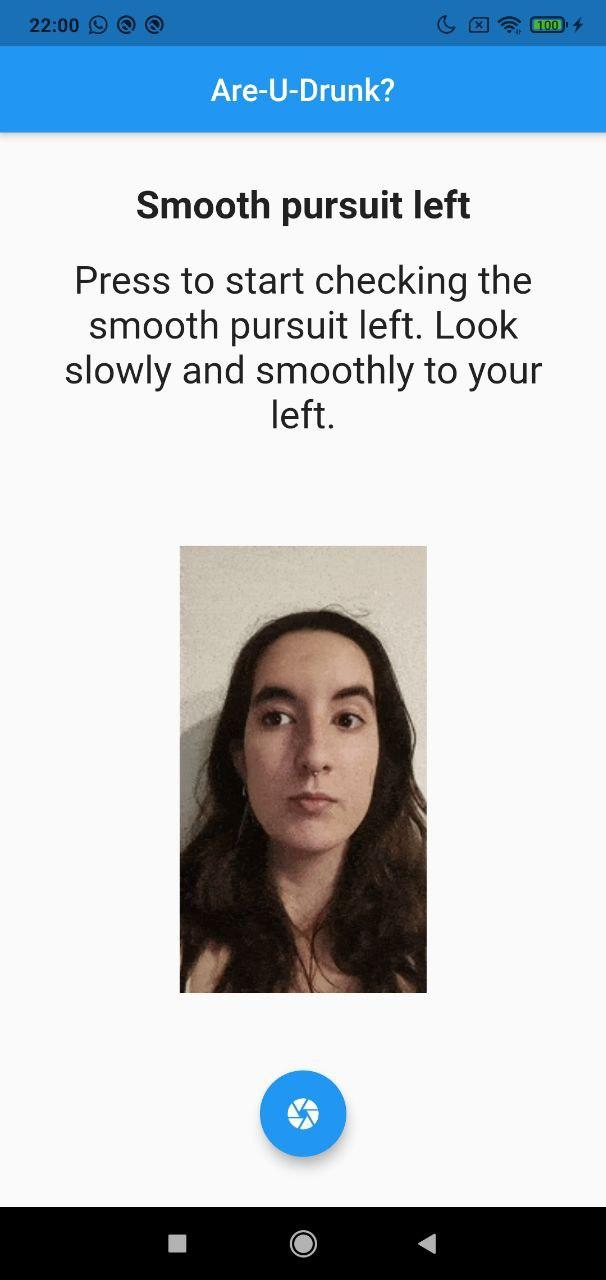
\includegraphics[width=0.5\textwidth]{./img/clueinfo.jpg}
      \caption{Page with information.}
      \label{clueinfo}
  \end{subfigure}\hfill
  \begin{subfigure}{0.33\textwidth}
      \centering
      
\includegraphics[width=0.5\textwidth]{./img/recordvideo.jpg}
      \caption{Page to record the video.}
      \label{recordvideo}
  \end{subfigure}
  \begin{subfigure}{0.33\textwidth}
      \centering
      
\includegraphics[width=0.5\textwidth]{./img/videopreview.jpg}
      \caption{Page to confirm video.}
      \label{videopreview}
  \end{subfigure}
\end{figure}

Code listing \ref{recordvideo} shows the page to record a clue. The user clicks the button to record and the phone starts recording and automatically stops after four seconds and redirects the user to the video preview screen, shown in listing \ref{videopreview}. Listing \ref{recording} shows the code to record the video and stop it automatically, and code listing \ref{preview} shows the call to the backend when the video is confirmed and the code to show a loading animation while the backend is proccessing the request.

\begin{lstlisting}[language=flutter, basicstyle=\small, label={recording}, caption={Code to record video automatically}, captionpos=b]
await _initializeControllerFuture;
await _controller.startVideoRecording();
await Future.delayed(const Duration(seconds: 4), () {});
final image = await _controller.stopVideoRecording();
await Navigator.of(context).push(
MaterialPageRoute(builder: (context) => getNextPage(image.path)));
\end{lstlisting}

\begin{lstlisting}[language=flutter, basicstyle=\small, label={preview}, caption={Code to preview the recorded video}, captionpos=b]
context.loaderOverlay.show();
XFile video = XFile(widget.path);
String result = await callBackend(widget.endpoint, video);
context.loaderOverlay.hide();
\end{lstlisting}


The management of the response is shown in code listing \ref{management}.

\begin{lstlisting}[language=flutter, basicstyle=\small, label={management}, caption={Code to manage the response of the backend}, captionpos=b]
if (result == "fail") {
  failedClues += 1;
}

if (result == "undetected") {
  await Navigator.of(context).push(
    MaterialPageRoute(
        builder: (context) => EyeDetectionFailPage()),
  );
} else {
  if (failedClues < 2) {
    // If the picture was taken, display it on a new screen.
    await Navigator.of(context).push(
      MaterialPageRoute(
          builder: (context) => widget.getNextPage()),
    );
  } else {
    failedClues = 0;
    await Navigator.of(context).push(
      MaterialPageRoute(
          builder: (context) => DrunkPage()),
    );
  }
}
\end{lstlisting}
When the final result is obtained (eyes not detected, fail or pass), a similar screen to figure \ref{finalresult} is shown.

\begin{figure}[H]
  \centering
  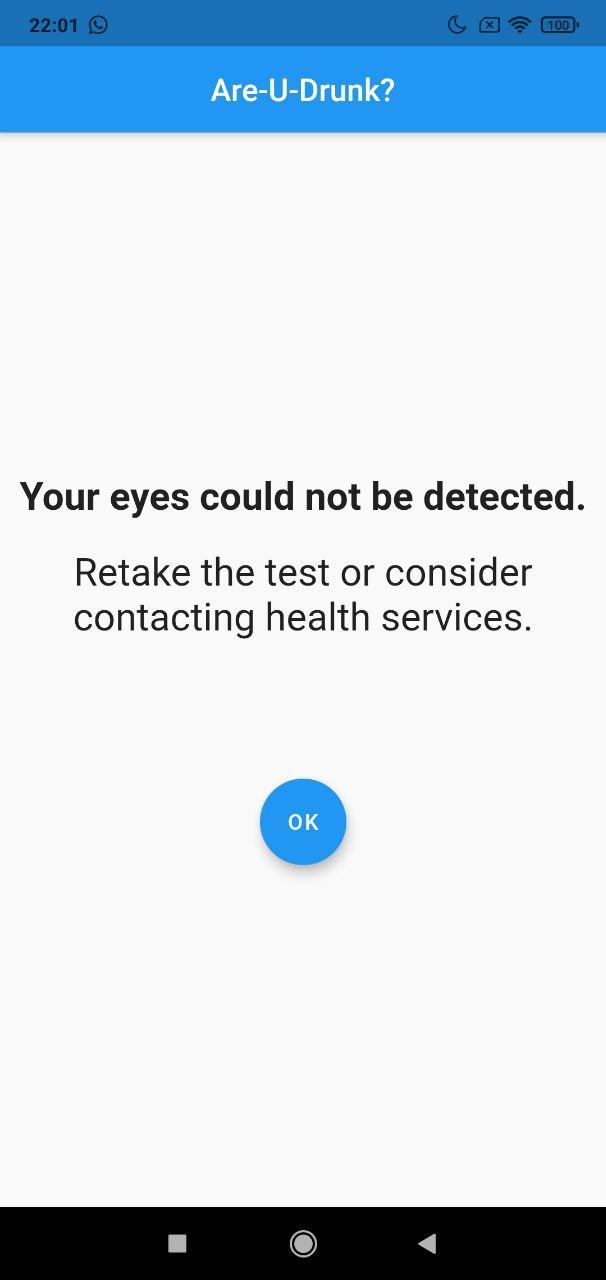
\includegraphics[width=0.22\textwidth]{./img/finalresult.jpg}
  \caption{Eyes not detected screen}
  \label{finalresult}
\end{figure}

\subsection{Server}

The server side uses Docker to host both the database and API. The interaction between the API and the database can be seen in Figure \ref{architecture}. This server is composed by an Application Programming Interface developed with Python and Gunicorn to receive data from the smartphone application and query the database, and a PostgreSQL database to store the videos recorded by de application. As previously mentioned, sqlalchemy is the toolkit used to query the database from the API.

Code listing \ref{docker-compose} shows the docker-compose.

\begin{lstlisting}[language=docker-compose-2, label={docker-compose}, caption={docker-compose}, captionpos=b]
version: '3'
services:
  database:
    image: "postgres:9.6.22-buster" # use 9.6.22-buster postgres version
    env_file:
      - database.env # configure postgres
    volumes:
      - database-data:/var/lib/postgresql/data/ # persist data even if container shuts down
    ports:
      - "60123:5432"
  backend:
    image: are_u_drunk_rest_api
    build: .
    ports:
      - "60321:5000"
    volumes:
      - clue-videos:/app/videos
volumes:
  database-data:
  clue-videos:
\end{lstlisting}

With this docker-compose, the database and backend services are created. The database service uses a volume to persist the data inserted when the service stops and starts again. The backend service uses a volume to store the videos recorded by the application and referenced in the database entries.


\begin{lstlisting}[language=docker, label={dockerfile}, caption={Dockerfile}, captionpos=b]
FROM python:3.8.11-slim-buster
RUN apt-get update && apt-get install -y libpq-dev gcc python3-dev musl-dev g++ libglib2.0-dev python3-opencv libopencv-dev
COPY requirements.txt /
RUN pip3 install -r /requirements.txt
RUN pip3 install ipython
COPY ./src /app
COPY ./run.sh /app
COPY ./gunicorn.conf.py /app
WORKDIR /app
ENV PYTHONPATH /app
RUN mkdir videos
ENTRYPOINT ["./run.sh"]
\end{lstlisting}

Code listing \ref{dockerfile} shows how the container is instantiated: a Python Docker image is used, the dependencies and requirements are installed, and finally, the code is copied to the container's root and \textit{run.sh} is set as the entry point. \textit{run.sh} initializes the app with the specified configuration in the Gunicorn config file. Also a directory named "videos" is created to store the videos recorded by the application.

As previously mentioned, Docker is used due to its ease to scale and deploy, and using the command shown in Figure \ref{dockercommand} the API and the backend can be set up in the environment (development and production).

\begin{lstlisting}[language=bash, mathescape=false, label={dockercommand}, caption={Commands to set the environment up}, captionpos=b]
$> docker-compose up --build d
\end{lstlisting}

\subsubsection{Database}

The database has been implemented following the schema shown in figure \ref{databaseschema}.

\begin{figure}[H]
    \centering
    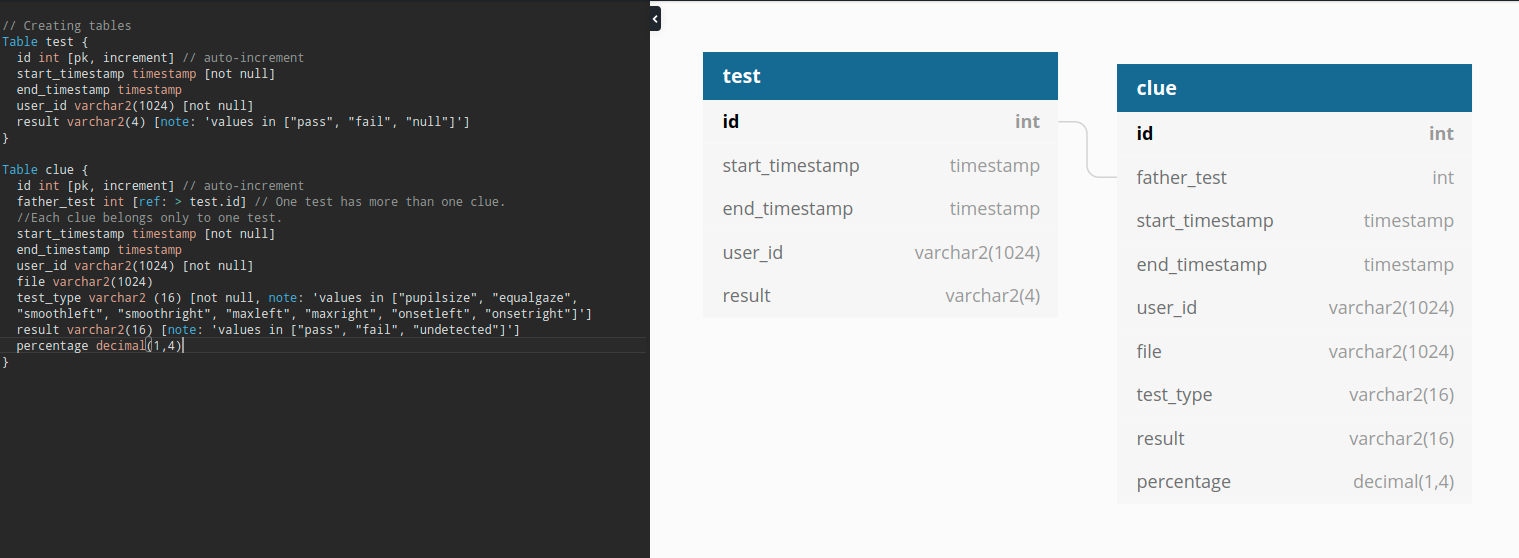
\includegraphics[width=0.95\textwidth]{./img/db.png}
    \caption{Database schema}
    \label{databaseschema}
\end{figure}

The entity \textit{Test} has an id (auto-incremental), a start timestamp (not nullable), an end timestamp (nullable), an unique identifier of the user who took the test (not nullable) and the result (nullable). The start timestamp is inserted as soon as the test begins and the end timestamp is updated as soon as the user ends each of the clue, so we could be able to trace if the user quits before ending the test and where. The result is inserted when the user finishes the last clue, either the 6th clue, the second failed clue or one in which the eyes are not recognized. With this implementation, if the user doesn't finish the test, the result is null and we could query the end timestamp to know in which clue the user quitted.

The entity \textit{Clue} has an id (auto-incremental), the id of the father test (not nullable), a start timestamp (not nullable), an end timestamp (nullable), an unique identifier of the user who took the test (not nullable), the path to the video file (nullable), the test type (not nullable), the result (nullable) and the percentage of success. The start timestamp is inserted as soon as the clue begins and the end timestamp is updated as soon as the user ends each of the clue, so we could be able to trace if the user quits while taking that clue. Therefore, the video file path is nullable since the user could quit and no video would be recorded. The result is inserted when the user finishes the clue. With this implementation, we could query either the result or the end timestamp to know if the user finished the clue.

\subsubsection{Python API}

The API consists of two classes to integrate with the database, seven different endpoints and seven different methods to analyze the video. The model definition for 'Clue' entity is shown in figure \ref{cluepy}.

  \begin{python}[basicstyle=\small, label={cluepy}, caption={Clue class in clue.py}, captionpos=b]
    class Clue(Base):
        __tablename__ = 'clue'
        id = Column(Integer, primary_key=True)
        father_test = Column(Integer, ForeignKey('test.id'))
        start_timestamp = Column(DateTime, nullable=False)
        end_timestamp = Column(DateTime, nullable=True)
        user_id = Column(String, nullable=False)
        file = Column(String, nullable=True)
        test_type = Column(String, nullable=False)
        result = Column(String, nullable=True)
        def __init__(self, father_test, start_timestamp, end_timestamp, user_id, file, test_type, result):
            self.father_test = father_test
            self.start_timestamp = start_timestamp
            self.end_timestamp = end_timestamp
            self.user_id = user_id
            self.file = file
            self.test_type = test_type
            self.result = result
  \end{python}

Out of the seven different endpoints, one is to initialize the test and the first clue and the six remaining are called when a clue ends. Figure \ref{maximumright} shows the endpoint called when the maximum deviation right is checked.

\begin{python}[label={maximumright}, caption={Enpoint to proccess the maximum deviation right}, captionpos=b]
  @app.route('/maximumright', methods=['POST'])
  def maximum_right():
    user = request.form['user']
    father_test_id = int(request.form['father_test_id'])
    time = datetime.utcnow()
    filename=f"{user}-{time.strftime('\%Y-\%m-\%d \%H:\%M:\%S')}-maximumright.mp4"
    request.files['media'].save(filename)
    perc = get_percentage(filename, 'right')
    if perc > LIMIT:
        return_result = "pass"
    elif perc == 0:
        return_result = "undetected"
    else:
        return_result = "fail"
    _insert_into_db(father_test_id=father_test_id, return_result=return_result, user=user, filename=filename,
                    current_clue_type="maximumright", time=time, percentage=perc)
    return {'result': return_result}
\end{python}

The six endpoints to proccess the clues follow the same structure: the request parameters are obtained (user who called the backend, the id assigned to the test that groups all the clues and the video recorded) and the video is saved, naming it after the user, the timestamp of the call and the type of clue. Then, the method to track and analyze the gaze and determine whether the clue is passed or not and depending on the result, the corresponding operations are performed in the database. Finally, the result is sent as a response. Figure \ref{getpercentage} shows the method previously mentioned. This code is based on Proctoring-AI project \cite{proctoringai}.


  \begin{python}[basicstyle=\footnotesize, caption={Method to track and analyze the gaze and determine whether the clue is passed or not}, captionpos=b, label={getpercentage}]
    def get_percentage(video, gaze):
    try:
        left_data_list = []
        right_data_list = []
        face_model = get_face_detector()
        landmark_model = get_landmark_model()
        left = [36, 37, 38, 39, 40, 41]
        right = [42, 43, 44, 45, 46, 47]
        cap = cv2.VideoCapture(video)
        kernel = np.ones((9, 9), np.uint8)
        while cap.isOpened():
            ret, img = cap.read()
            if ret:
                rects = find_faces(img, face_model)

                for rect in rects:
                    try:
                        shape = detect_marks(img, landmark_model, rect)
                    except cv2.error:
                        continue
                    mask = np.zeros(img.shape[:2], dtype=np.uint8)
                    mask, end_points_left = eye_on_mask(mask, left, shape)
                    mask, end_points_right = eye_on_mask(mask, right, shape)
                    mask = cv2.dilate(mask, kernel, 5)
                    eyes = cv2.bitwise_and(img, img, mask=mask)
                    mask = (eyes == [0, 0, 0]).all(axis=2)
                    eyes[mask] = [255, 255, 255]
                    mid = int((shape[42][0] + shape[39][0]) // 2)
                    eyes_gray = cv2.cvtColor(eyes, cv2.COLOR_BGR2GRAY)
                    threshold = 75
                    _, thresh = cv2.threshold(eyes_gray, threshold, 255, cv2.THRESH_BINARY)
                    thresh = process_thresh(thresh)
                    contouring(thresh[:, 0:mid], mid, img, end_points_left, False, right_data_list, left_data_list)
                    contouring(thresh[:, mid:], mid, img, end_points_right, True, right_data_list, left_data_list)
                    for (x, y) in shape[36:48]:
                        cv2.circle(img, (x, y), 2, (255, 0, 0), -1)
            else:
                break
        cap.release()
        cv2.destroyAllWindows()
        try:
            if gaze == 'right':
                result = count_wrong_meassurements(right_data_list, True) / len(right_data_list)
            else:
                 result = count_wrong_meassurements(left_data_list) / len(left_data_list)
            return 1 - result
        except ZeroDivisionError:
            return 0
    except cv2.error:
        logger.exception("Exception detecting eyes")
        return 0
  \end{python}

In the get\_percentage method, two arrays are firstly created to store the points obtained from the eyes, the face detector and landmark model are instantiated and the landmark coordinates for the left and right eyes are harcoded. These landmark coordinates are obtained from the Dlib facial keypoints. Then, the video is analyzed frame by frame, detecting firstly the eyes with the eye\_on\_mask method and then detecting the eye position with the contouring method. All of the positions are stored in the corresponding data list and when the video is completely analyzed, the percentage of positions that are invalid is calculated. A position is considered invalid when the previous one is greater in the case of a left gaze and smaller in the case of a right gaze. If no data is stored in the list, eyes have not been detected and the method returns zero.

\subsubsection{Deployment}

This project has been uploaded to a server provided by de University of Granada \cite{ugr}. For this purpose, the requests have been proxied through Nginx \cite{nginx}. This is also useful to isolate the Are-U-Drunk project from the rest of the projects hosted in the server. To deploy the system, Docker is required in the server. Once this requirement is met, the application has to be downloaded from the repository and copied to the server. Then, the Gunicorn config file has to be modified to set the new path for the requests and using the command shown in listing \ref{dockercomposeup} the containers for the services start working.

\begin{lstlisting}[label={dockercomposeup}, caption={Command to start the containers}, captionpos=b]
docker-compose up
\end{lstlisting}

The database is created by means of two scripts, one for each table. Listing \ref{dbscript} shows the script used to create the table for the tests. A database.env file has to be created to configure secure credentials to access the database.

\begin{lstlisting}[label={dbscript}, caption={Script to create the table for the tests}, captionpos=b]
SET statement_timeout = 0;
SET lock_timeout = 0;
SET idle_in_transaction_session_timeout = 0;
SET client_encoding = 'UTF8';
SET standard_conforming_strings = on;
SELECT pg_catalog.set_config('search_path', '', false);
SET check_function_bodies = false;
SET xmloption = content;
SET client_min_messages = warning;
SET row_security = off;
SET default_tablespace = '';
CREATE TABLE public.test (
    id integer NOT NULL,
    start_timestamp timestamp without time zone NOT NULL,
    end_timestamp timestamp without time zone,
    user_id character varying NOT NULL,
    result character varying
);
ALTER TABLE public.test OWNER TO cdg;
CREATE SEQUENCE public.test_id_seq
    START WITH 1
    INCREMENT BY 1
    NO MINVALUE
    NO MAXVALUE
    CACHE 1;
ALTER TABLE public.test_id_seq OWNER TO cdg;
ALTER SEQUENCE public.test_id_seq OWNED BY public.test.id;
ALTER TABLE ONLY public.test ALTER COLUMN id SET DEFAULT nextval('public.test_id_seq'::regclass);
ALTER TABLE ONLY public.test
    ADD CONSTRAINT test_pkey PRIMARY KEY (id);
\end{lstlisting}

Finally, the path to the application is added to nginx to redirect the request and the service is restarted. Listing \ref{nginxcode} shows this change.

\begin{lstlisting}[label={nginxcode}, caption={Nginx configuration file}, captionpos=b, mathescape]
server {
	listen 80 default_server;
	listen [::]:80 default_server;
	server_name _;
	return 301 https://hostrequest_uri;

}

server {
	listen 443 ssl default_server;
	listen [::]:443 ssl default_server;
	...
  location /are_u_drunk_backend {
    proxy_pass  http://localhost:60321;
    proxy_set_header Host host;
    proxy_set_header X-Real-IP remote_addr;
    proxy_set_header X-Forwarded-For proxy_add_x_forwarded_for;
	}
  ...
}
\end{lstlisting}

\newpage
\section{Evaluation}
\label{discussion}

\subsection{Methodology}

The mobile application 'Are-U-Drunk?' has been tested with 8 people, aged from 18 to 58, 4 female and 8 male. The 8 participants were tested using the application once before drinking different amounts of alcohol and once after drinking it. If any inconvenience happpened (eyes could not be detected for any reason), the test was repeated. This mobile testing happened when and were the participant desired any time before drinking and 15-30 minutes after drinking. The day after the last mobile test, a form was provided to take a System Usability Scale (SUS) \cite{sus} test.

\subsection{Usability}

To test the usability of the system, SUS \cite{sus} has been used. This test is composed by 10 statements, in each of which the respondent states how they feel about the statement from 1 to 5, being 1 strongly disagree and 5 strongly agree. The 10 statements are the following.

\begin{itemize}
  \item I think that I would like to use this system frequently.
  \item I found the system unnecessarily complex.
  \item I thought the system was easy to use.
  \item I think that I would need the support of a technical person to be able to use this system.
  \item I found the various functions in this system were well integrated.
  \item I thought there was too much inconsistency in this system.
  \item I would imagine that most people would learn to use this system very quickly.
  \item I found the system very cumbersome to use.
  \item I felt very confident using the system.
  \item I needed to learn a lot of things before I could get going with this system.
\end{itemize}

\begin{figure}[h!]
  \centering
  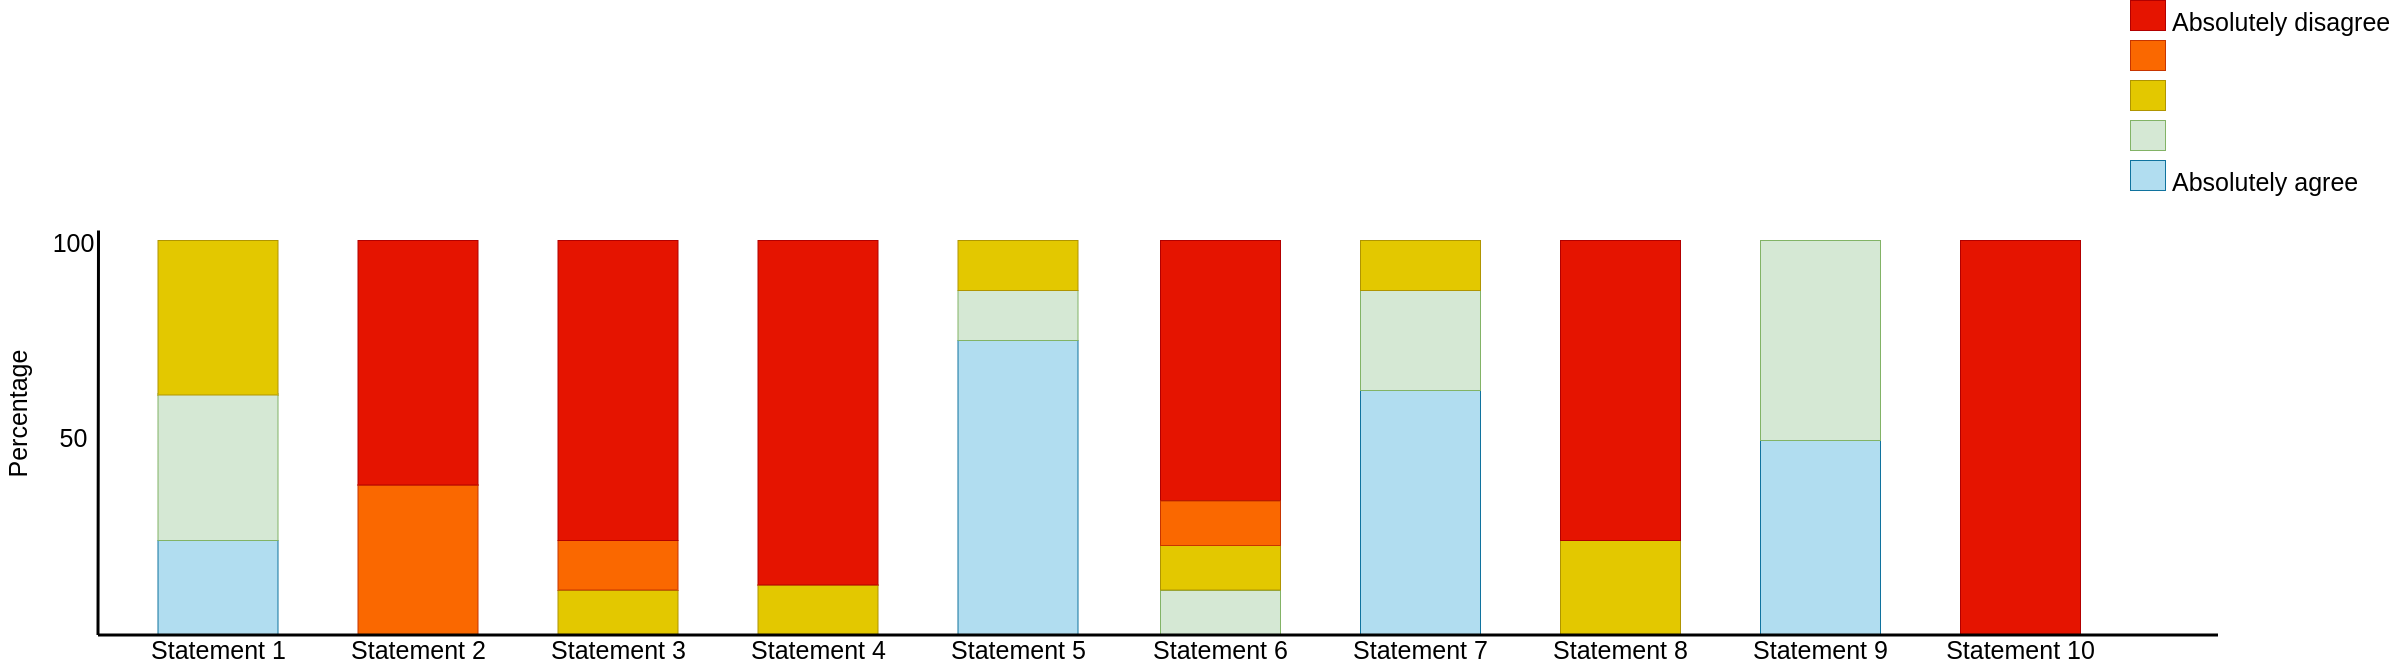
\includegraphics[angle=90, height=23cm,keepaspectratio]{./img/SUS.png}
  \caption{System Usability Scale responses' graph}
  \label{susgraph}
\end{figure}

Figure \ref{susgraph} represents the results. When asking if the participant would like to use this application frequently, 25\% strongly agreed, 37.5\% agreed and 37.5\% were neutral about the question. The system was not unnecessarily complex, 62.5\% of the users strongly disagreed about the application being complex and 37.5\% disagreed. 75\% of the participants strongly agreed the system was wasy to use, 12.5\% agreed and 12.5\% were neutral. Most of the participants, 87.5\%, strongly disagreed they would need the support of a technical person to be able to use the application and 12.5\% were neutral. When asking if the user found the various functions in the system were well integrated, 75\% strongly agreed, 12.5\% agreed and 12.5\% were neutral. The participants' opinions on whether there was too much inconsistency in this application are: 62.5\% strongly disagreed, 12.5\% disagreed, 12.5\% were neutral and 12.5\% agreed. 62.5\% of the users strongly agreed that most people would learn to use this system very quickly, 25\% agreed and 12.5\% were neutral. 75\% strongly disagreed the system was very cumbersome to use while 25\% was neutral about it. 50\% agreed they felt very confident using the application and 50\% strongly agreed. Finally, 100\% strongly disagreed they needed to learn a lot of thing before get going with the tests.

\subsection{Performance}



% Please add the following required packages to your document preamble:
% \usepackage{multirow}
\begin{table}[h!]
  % Please add the following required packages to your document preamble:
  % \usepackage{multirow}
  % Please add the following required packages to your document preamble:
  % \usepackage{multirow}
  % Please add the following required packages to your document preamble:
% \usepackage{multirow}
\begin{tabular}{|l|l|l|l|l|l|l|}
\hline
Participant                    & Gender                  & Age                 & Amount drank                                                                                  & Samples  & \begin{tabular}[c]{@{}l@{}}Before or \\ after \\ drinking\end{tabular} & Result     \\ \hline
\multirow{4}{*}{Participant 1} & \multirow{4}{*}{Female} & \multirow{4}{*}{25} & \multirow{4}{*}{Half a glass of wine}                                                         & Sample 1 & Before                                                                 & Null       \\ \cline{5-7}
                               &                         &                     &                                                                                               & Sample 2 & Before                                                                 & Fail       \\ \cline{5-7}
                               &                         &                     &                                                                                               & Sample 3 & After                                                                  & Undetected \\ \cline{5-7}
                               &                         &                     &                                                                                               & Sample 4 & After                                                                  & Fail       \\ \hline
\multirow{3}{*}{Participant 2} & \multirow{3}{*}{Male}   & \multirow{3}{*}{23} & \multirow{3}{*}{Half a glass of wine}                                                         & Sample 1 & Before                                                                 & Fail       \\ \cline{5-7}
                               &                         &                     &                                                                                               & Sample 2 & Before                                                                 & Fail       \\ \cline{5-7}
                               &                         &                     &                                                                                               & Sample 3 & After                                                                  & Fail       \\ \hline
\multirow{2}{*}{Participant 3} & \multirow{2}{*}{Male}   & \multirow{2}{*}{54} & \multirow{2}{*}{\begin{tabular}[c]{@{}l@{}}Two beers and \\ two glasses of wine\end{tabular}} & Sample 1 & Before                                                                 & Fail       \\ \cline{5-7}
                               &                         &                     &                                                                                               & Sample 2 & After                                                                  & Fail       \\ \hline
\multirow{3}{*}{Participant 4} & \multirow{3}{*}{Male}   & \multirow{3}{*}{18} & \multirow{3}{*}{Half a glass of wine}                                                         & Sample 1 & Before                                                                 & Fail       \\ \cline{5-7}
                               &                         &                     &                                                                                               & Sample 2 & After                                                                  & Undetected \\ \cline{5-7}
                               &                         &                     &                                                                                               & Sample 3 & After                                                                  & Fail       \\ \hline
\multirow{2}{*}{Participant 5} & \multirow{2}{*}{Female} & \multirow{2}{*}{53} & \multirow{2}{*}{A glass of wine}                                                              & Sample 1 & Before                                                                 & Fail       \\ \cline{5-7}
                               &                         &                     &                                                                                               & Sample 2 & After                                                                  & Fail       \\ \hline
\multirow{2}{*}{Participant 6} & \multirow{2}{*}{Male}   & \multirow{2}{*}{58} & \multirow{2}{*}{\begin{tabular}[c]{@{}l@{}}One and a half \\ rum and coke\end{tabular}}       & Sample 1 & Before                                                                 & Fail       \\ \cline{5-7}
                               &                         &                     &                                                                                               & Sample 2 & After                                                                  & Fail       \\ \hline
\multirow{2}{*}{Participant 7} & \multirow{2}{*}{Female} & \multirow{2}{*}{54} & \multirow{2}{*}{Half a rum and coke}                                                          & Sample 1 & Before                                                                 & Fail       \\ \cline{5-7}
                               &                         &                     &                                                                                               & Sample 2 & After                                                                  & Fail       \\ \hline
\multirow{3}{*}{Participant 8} & \multirow{3}{*}{Female} & \multirow{3}{*}{22} & \multirow{3}{*}{A beer}                                                                       & Sample 1 & Before                                                                 & Fail       \\ \cline{5-7}
                               &                         &                     &                                                                                               & Sample 2 & After                                                                  & Undetected \\ \cline{5-7}
                               &                         &                     &                                                                                               & Sample 3 & After                                                                  & Fail       \\ \hline
\end{tabular}
\caption{Subjects and samples of the application}
\label{subjects}
\end{table}

As Table \ref{subjects} shows, gender and age have been considered in the study participants, having an equal percentage of male and female people and a wide age range. Most of the tests are failed, three did not detect the eyes and one was quitted. The results of the tests were mainly 'fail'. Querying the database with the query shown in Listing \ref{dbquery}, we obtain the following data: 4 out of the 19 tests taken by all of the participants finished with only two clues, 6 finished with 3 clues, 5 finished with 4 clues and 6 finished in the 6th and last clue.

\begin{lstlisting}[caption={SQL query used to group the tests by the number of clues taken}, captionpos=b, label={dbquery}]
select acc, count(*) from (select count(*) as clues from public.clue group by father_test having count(*) > 1) as acc group by acc
\end{lstlisting}

The percentages of accuracy of eye movement in the failed clues were between 41.91\% and 56\% when the first two clues are failed. When the tests stopped at the third clue, the percentages varied from 50.86\% to 60\%, when the fourth was the last clue, the percentages were between 42.86\% and 60\% and finally, if the test finished with a failed last clue, the percentages varied from 50.36\% to 58.9\%. Some of the failed clues' videos were too dark, which may have caused the algorithm not to detect and track the eyes properly. Glasses also appear to affect the detection since all of the clues with a result of 'undetected' were taken with glasses. This may also affect the tracking of the eyes, but further research has to be done to affirm this. Furtuhermore, some of the videos were recorded too fast, meaning this that the eyes were moving faster than expected. After drinking, then number of passed clues was lower than the previous test when the participant was sober.

\newpage
\section{Conclusions}
\label{conclusions}

In this section, the objectives previously set will be analyzed. Furthermore, possible future work will be defined.

\subsection{Achieved objectives}

\begin{itemize}
  \item \textbf{Main goal: to develop a system to automatically assess a person’s drunkness based on the analysis of their eye(s) movement.} A complete system, composed by a mobile phone (camera and internet connection included) and a backend hosted in a server, has been developed and the functionality and usability of it has been tested by a small sample of people.
  \item \textbf{Secondary goals:}
  \begin{itemize}
    \item \textbf{To design a system that detects and tracks the user’s eyes and analyzes them in search of horizontal nystagmus movements.} The designed architecture is composed by the mobile application that, according to the proposed requirements, will record some videos to detect and track the eyes, send them to a server and proccess them.
    \item \textbf{To develop a system that detects and tracks the user’s eyes and analyzes them in search of horizontal nystagmus movements.} This goal has been achieved by means of analyzing the videos sent by the user and tracking the position of the eyes for every frame to check the movement looking for horizontal nystagmus movements.
    \item \textbf{To evaluate and test the previously mentioned system.} A small sample of people used the designed and developed application before and after drinking. These people have also taken an usability test to check the ease of use of the application.
  \end{itemize}
\end{itemize}

\subsection{Future work}

The mobile application 'Are-U-Drunk' could be improved in many ways. Some of the proposals for future work are:

\begin{itemize}
  \item Improve the algorith to be resilient to different illumination levels. This will result in a more accurate test result since the eyes and the gaze could be detected in more complicated scenarios.
  \item Create and train a new model from scrath. This could help the algorithm detect the eyes faster and better.
  \item Improve the user experience by features like clinging or vibrating when the camera stops recording.
  \item Link a video with a deeper explanation about the test and the clues so the user knows exactly how the video must be recorded.
\end{itemize}

\newpage
\begin{appendices}

\section{\textbf{State of the Art Matrix}}
\label{appendix:matrix}
\url{https://docs.google.com/spreadsheets/d/1mtM97CYdcI7DFjK2QBlT6idoHjkSppf8CLmN4FE_H24/edit?usp=sharing}

\begin{figure}[H]
  \centering
      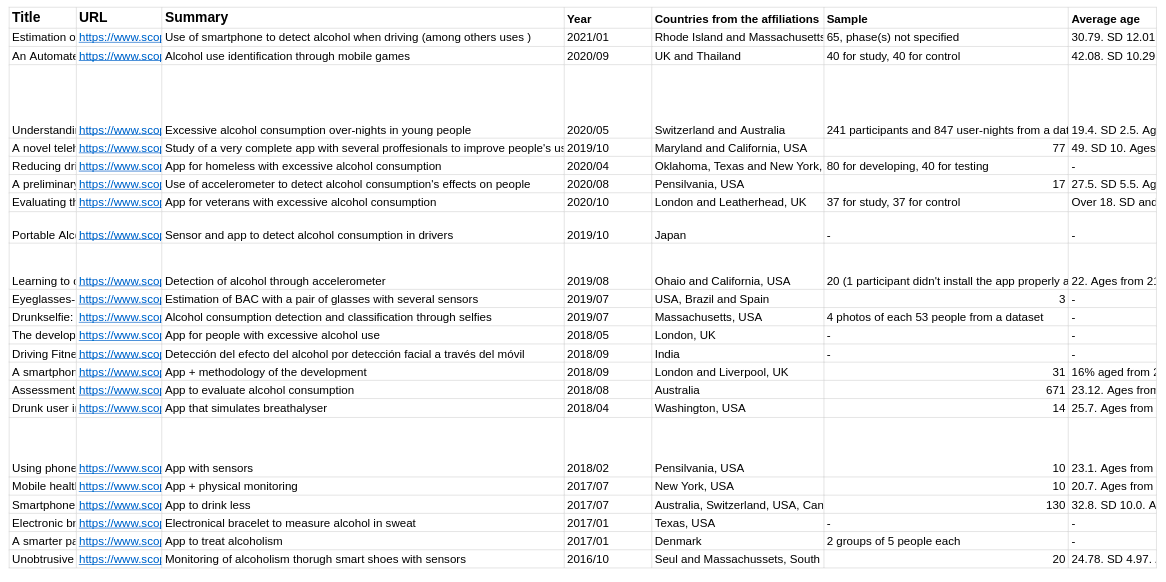
\includegraphics[width=1\textwidth]{./img/matriz.png}
      \caption{Preview of the State of the Art Matrix}
      \label{matrix}
\end{figure}

\end{appendices}



\newpage
\bibliographystyle{IEEEtran}
\bibliography{refs}
\doclicenseThis

\end{document}
